\chapter{基于波动随机照明的透过散射介质超OME范围成像}\label{chap:5}

非侵入式光学成像在从生物成像技术\cite{zhao_non-invasive_2001,artzi_vivo_2011}到光学检测\cite{kozloff_non-invasive_2009}的各个领域都有重要应用。但是,不均匀的样品(例如生物组织)会散射光,从而导致探测器上出现复杂的散斑图案\cite{Goodman1976,Bender}。
随着穿透深度的增加,从散射光中分离出少量的弹道光成为一个很大的挑战\cite{Abramson1978,huang_optical_1991}。多年来,科研人员提出了许多方法通过利用或抑制散射光来克服透过散射介质实现非入侵成像的问题。随着SLM的发展,许多方法已经被提出来实现控制和操纵散射光\cite{Mosk2012,rotter_light_2017}。目前,已经提出了几种技术通过使用反馈信号优化入射光波前进而实现聚焦,以重新形成一个焦点,然后利用扫描的方式实现成像\cite{Vellekoop2007,Horstmeyer2015}。这些技术通常需要途径至散射层的两侧获取反馈信号以优化波前,这些条件极大地限制了它们在实际场景中的应用。
为了克服这个问题,已经提出了基于波前整形和各种反馈信号(例如荧光或超声信号)的其他策略\cite{Horstmeyer2015,Katz2019,Popoff2010,Hofer2019},实现波前整形。然而,这些方法要么需要较长的采集时间,要么仅限于小视场。
另一方面,还提出了几种利用角散斑相关性的技术\cite{bertolotti_non-invasive_2012,katz_non-invasive_2014},即OME\cite{Freund1988,Yllmaz2019,Osnabrugge},用于对隐藏在散射介质后面的物体进行成像。这些方法计算散斑图案的自相关,其本质上利用散斑的自相关与隐藏目标的自相关相同,并使用相位恢复算法从自相关重建对象图像。虽然这些方法速度很快,但它们的成像范围仍然受到OME范围的限制。前面章节中,我们对基于OME下的散斑成像进行了原理介绍和实验验证。

线性荧光广泛应用于生物学和生物医学科学\cite{Ruan2020,Lichtman2005,mangeat_super_resolved_2021}。 它能够对细胞、亚细胞或分子成分进行成像,并具有空间分辨率高、对比度高、速度快的优点。近年来,许多技术允许使用荧光通过散射介质进行聚焦和成像。
即便如此,这些方法要么依赖于引导星 \cite{Hhorstmeyer} 的使用,仅限于OME范围 \cite{hofer_wide_2018},要么需要表征散射介质 \cite{boniface_non_invasive_2020}。

在本章,我们提出了一种新型的成像方法,该方法使用简单地利用旋转漫射器生成的波动随机散斑照明,允许透过散射介质在一定深度上远远超出OME范围的进行非侵入性成像。当随机照明散斑产生后,每个荧光点光源都会在探测器上产生独特的散斑图案,我们称其为“散斑指纹”。相机所捕获的每张图像都是来自不同荧光点光源的所产生的散斑指纹的非相干总和。当随机照明随着旋转器改变时,探测器上所接收的散斑的各个散斑指纹的权重随之改变。为了检索每个单独的指纹,我们在随机改变光照的同时捕获一组图像,并使用非负矩阵分解 (Non-negative Matrix Factorization,NMF) 算法对采集的数据进行去混叠。随后,通过探索指纹之间的相关性,使用指纹重建最终图像。为了验证该技术的有效性,我们通过实验证明了我们在荧光珠和连续荧光物体上的非侵入性成像方法。

\section{基于波动随机照明的透过散射介质超OME范围成像基本原理}

\begin{figure}[htp]
	\centering
	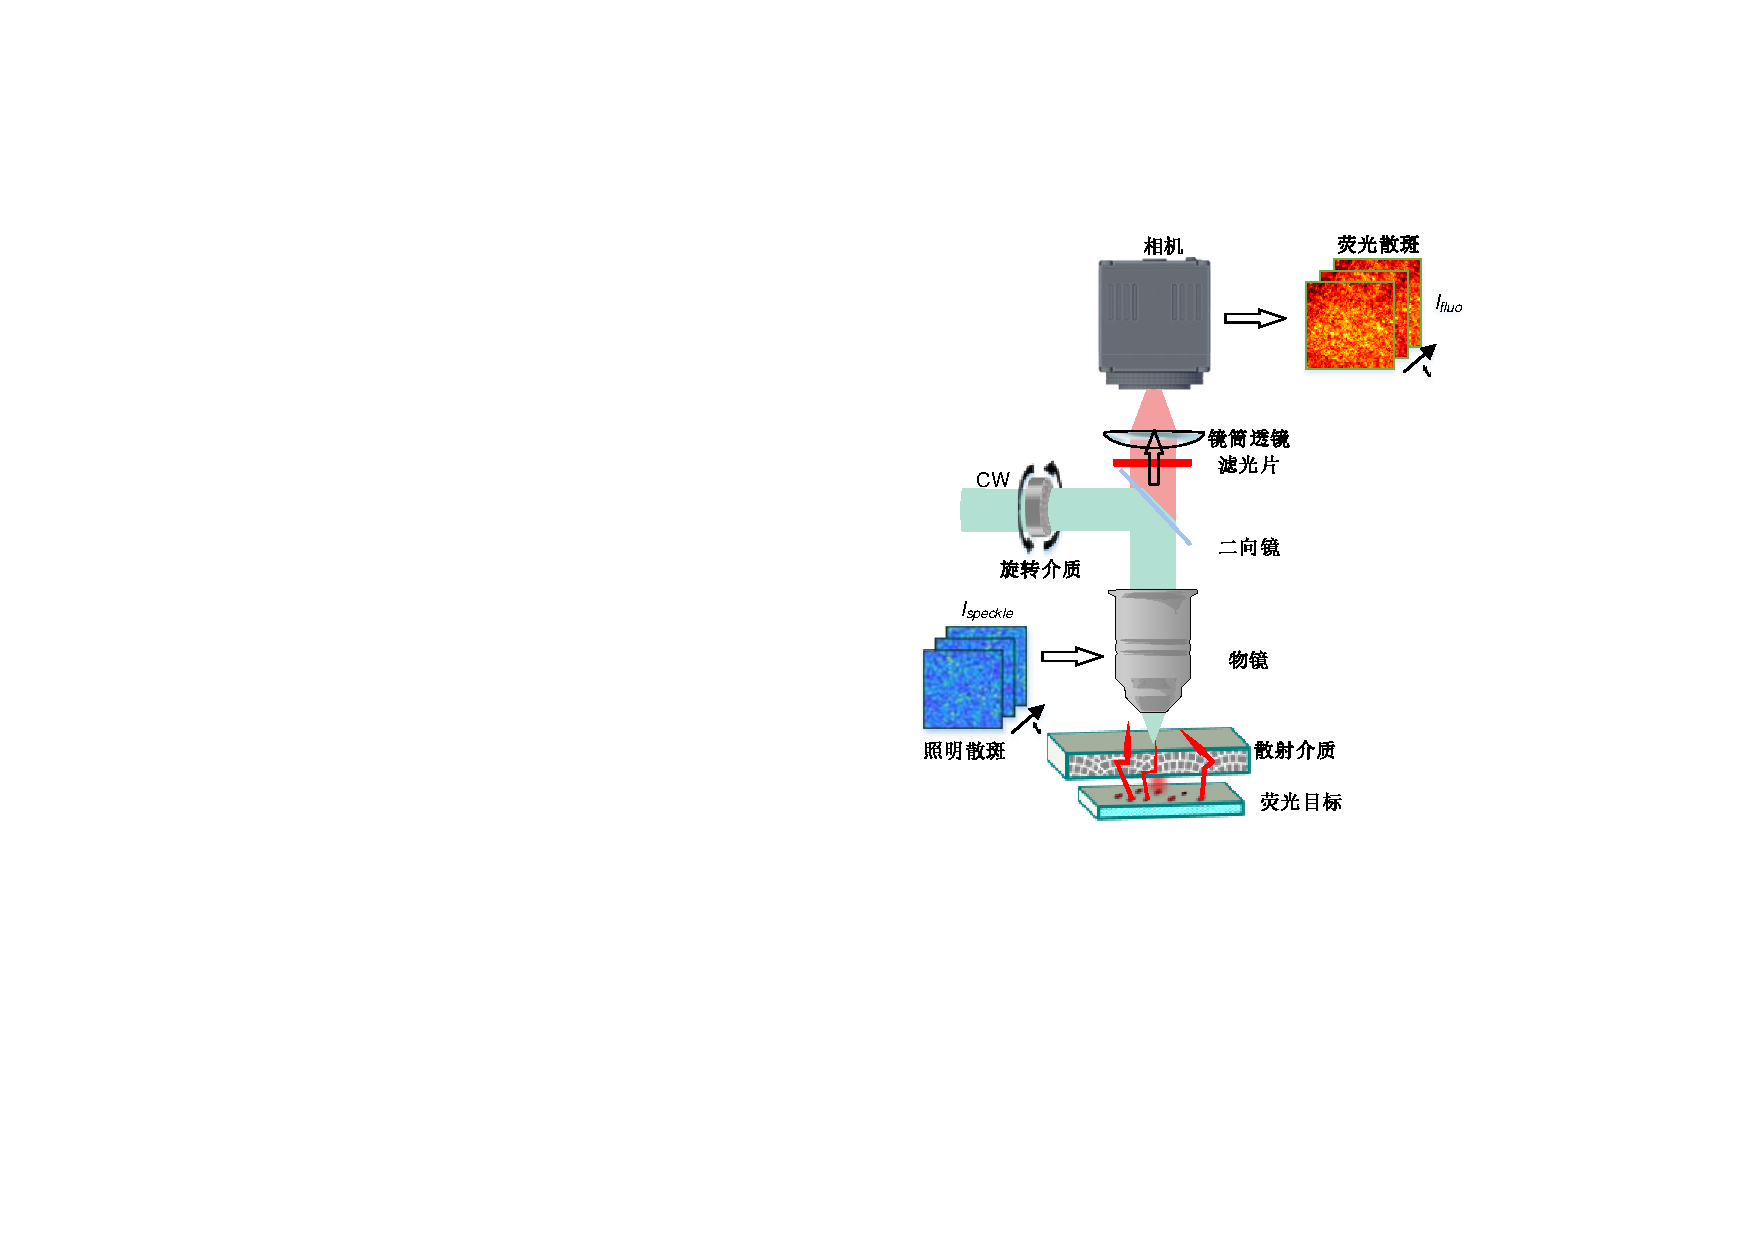
\includegraphics[scale=0.75]{C5.fig1}
	\caption{非入侵成像系统示意图}
	\label{fig:5.1}
\end{figure}

非入侵成像系统如图\ref{fig:5.1}所示。当激光通过旋转漫反射器时,入射激光被添加了随机相位实现了入射激光的随机调制,进而调制光透过散射介质产生了未知的随机散斑,未知的散斑照明目标。利用随机散斑照明目标后,目标产生自身的激发光,激发光传播并通过散射介质,产生散斑最终被相机所接收,此时相机所获得的散斑为不同散斑指纹的非相干总和。尽管捕获的图像对比度低、随机且看似无信息,但它们包含来自对象独立点光源的所有散斑指纹,且其各自的权重随着随机照明的改变具有时间的多样性。此外,OME范围内的独立点光源将在相机上产生相关但平移的散斑指纹 \cite{Freund1988},而OME范围外的点光源将产生完全不相关的散斑指纹。对于给定的散斑照明,捕获的图像 $I_{\textsl{fluo}}$ 可以表示为具有不同权重的散斑指纹的线性叠加。因此,相机图像$I_{\textsl{fluo}}$由下式给出:

\begin{equation}
\begin{aligned}
I_{fluo}(r,t) = \sum^{P}_{k=1} w_{k}(r) h_{k}(t),
\label{eq:5.1}
\end{aligned}
\end{equation}
其中,$I_{fluo}(r,t)$为对应于第$t$次照明时相机所接收到低对比度散斑,$r$为空间坐标,$w_{k}(r)$为第$k$个独立点光源所对应的散斑指纹,$h_{k}(t)$为第$t$次照明时第$k$个独立点光源所接收到的激光光的强度,$P$为系统中独立点光源的数量。

当拥有足够多的随机散斑照明时,就可以采集到足够的低对比度散斑图案,通过NNF对散斑集进行去混叠,获得各自点光源的散斑指纹。然后利用,指纹重建算法实现最终图像的重建。整体流程下所示;
\begin{algorithm2e}[h!]
\DontPrintSemicolon
\SetAlgoLined
\KwInput{系列散斑图案, $I_{fluo}(r,t)$.}
\KwOutput{隐藏目标的图像, $O^{Global}$.}
从系列数据集$I_{fluo}(r,t)$估计系统的秩($\rho$).\;

通过去混叠算法恢复散斑指纹($w_{i}$).\;

\For{$k=1,...,\rho$}{
在指纹$w_{k}$和其余所有的指纹($w_{i\neq k}$)之间进行成对去卷积运算.\;

获取位于与散斑指纹$w_{k}$所对应的独立点光源同一OME范围内的独立点光源之间的相对位置.\;

获得局部重建结果($O_{k}$).\;
}

将不同区域的局部重建结果($O_{k}$)合成全局重建结果($O^{Global}$).\;

\caption{非入侵图像重建流程}
\label{alg:a1}
\end{algorithm2e}

\subsection{散斑指纹去混叠}

\begin{figure}[htp]
	\centering
	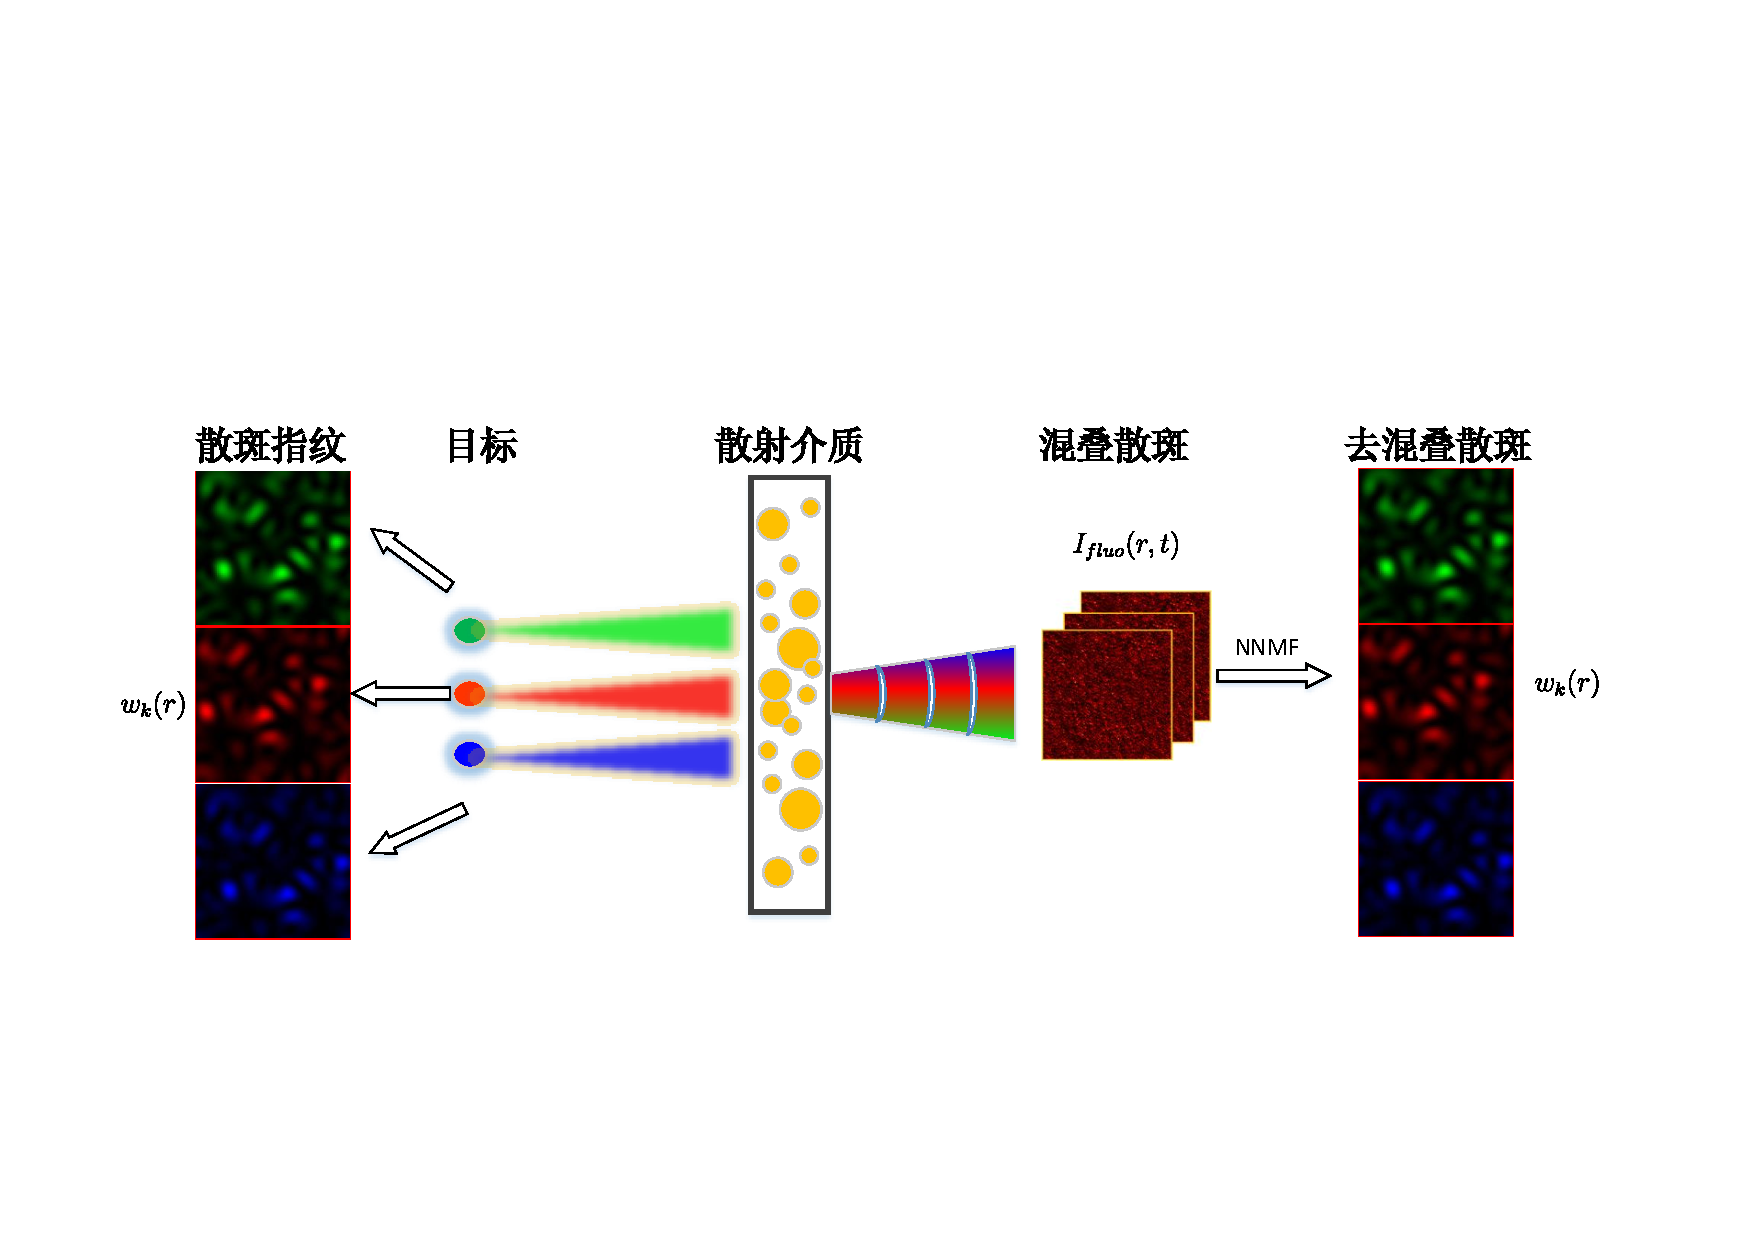
\includegraphics[scale=0.5]{C5.fig4}
	\caption{散斑去混叠示意图}
	\label{fig:5.4}
\end{figure}

如图\ref{fig:5.4}所示,独立点光源所对应的各自的散斑指纹一定,当我们使用散斑照明时,获得一些列混叠散斑。如何从一些混叠散斑中恢复出每个独立点光源的散斑指纹,将在接下来部分描述。

如公式(\ref{eq:5.1})所示,当使用随机照明时,$h_{k}(t)$随着照明的改变该随之变化。因为照明强度和散斑指纹的非负性,我们可以通过非线性优化的方式求得$w_{k}(r)$,即:

\begin{equation}
	\begin{aligned}
\min_{W>0,H>0} \Arrowvert I -WH\Arrowvert_F^{2},
\label{eq:5.2}
\end{aligned}
\end{equation}
其中,$\vert\vert M\vert\vert_F = \sqrt{\sum_i\sum_j \vert M_{ij}\vert^2}$为Frobenius矩阵范数。公式(\ref{eq:5.2})最小化问题可以表述为一个低秩分解问题。$I \in \mathbb{R}_{+}^{r \times t} $包含所有的散斑图案$I_{fluo}(r,t)$,$I \in \mathbb{R}_{+}^{r \times t}$ 可以被近似为两个实数矩阵$W \in \mathbb{R}_{+}^{r \times \rho}$ 和$H \in \mathbb{R}_{+}^{\rho \times t}$。
矩阵$W \in \mathbb{R}_{+}^{r \times \rho}$为指纹矩阵,$H \in \mathbb{R}_{+}^{\rho \times t}$为时间矩阵,其中 $r$ 是像素,$\rho$ 是 $I$矩阵所估计的秩,$t$ 表示散斑帧数。由于收集到的图像和混合指纹都具有非负性,这个问题正好对应于NMF优化问题。
NMF算法常用于去混叠场景,例如结构性成像\cite{boniface_non_invasive_2020}和功能性成像\cite{Moretti2020a,Pegard2016, Pnevmatikakis2016}等,NMF去混叠过程如图\ref{fig:5.2}所示。
在数据矩阵去混叠之前,我们需要对所获得的相机散斑进行滤波,去除散斑的轮廓噪声,在傅里叶域中移除低频信号,如图\ref{fig:5.3}所示。在NMF算法的运行过程前,我们需要确定$\rho$,该参数可以通过最小化NMF的均方根残差作为秩的函数来从数据中估计。

\begin{figure}[htp]
	\centering
	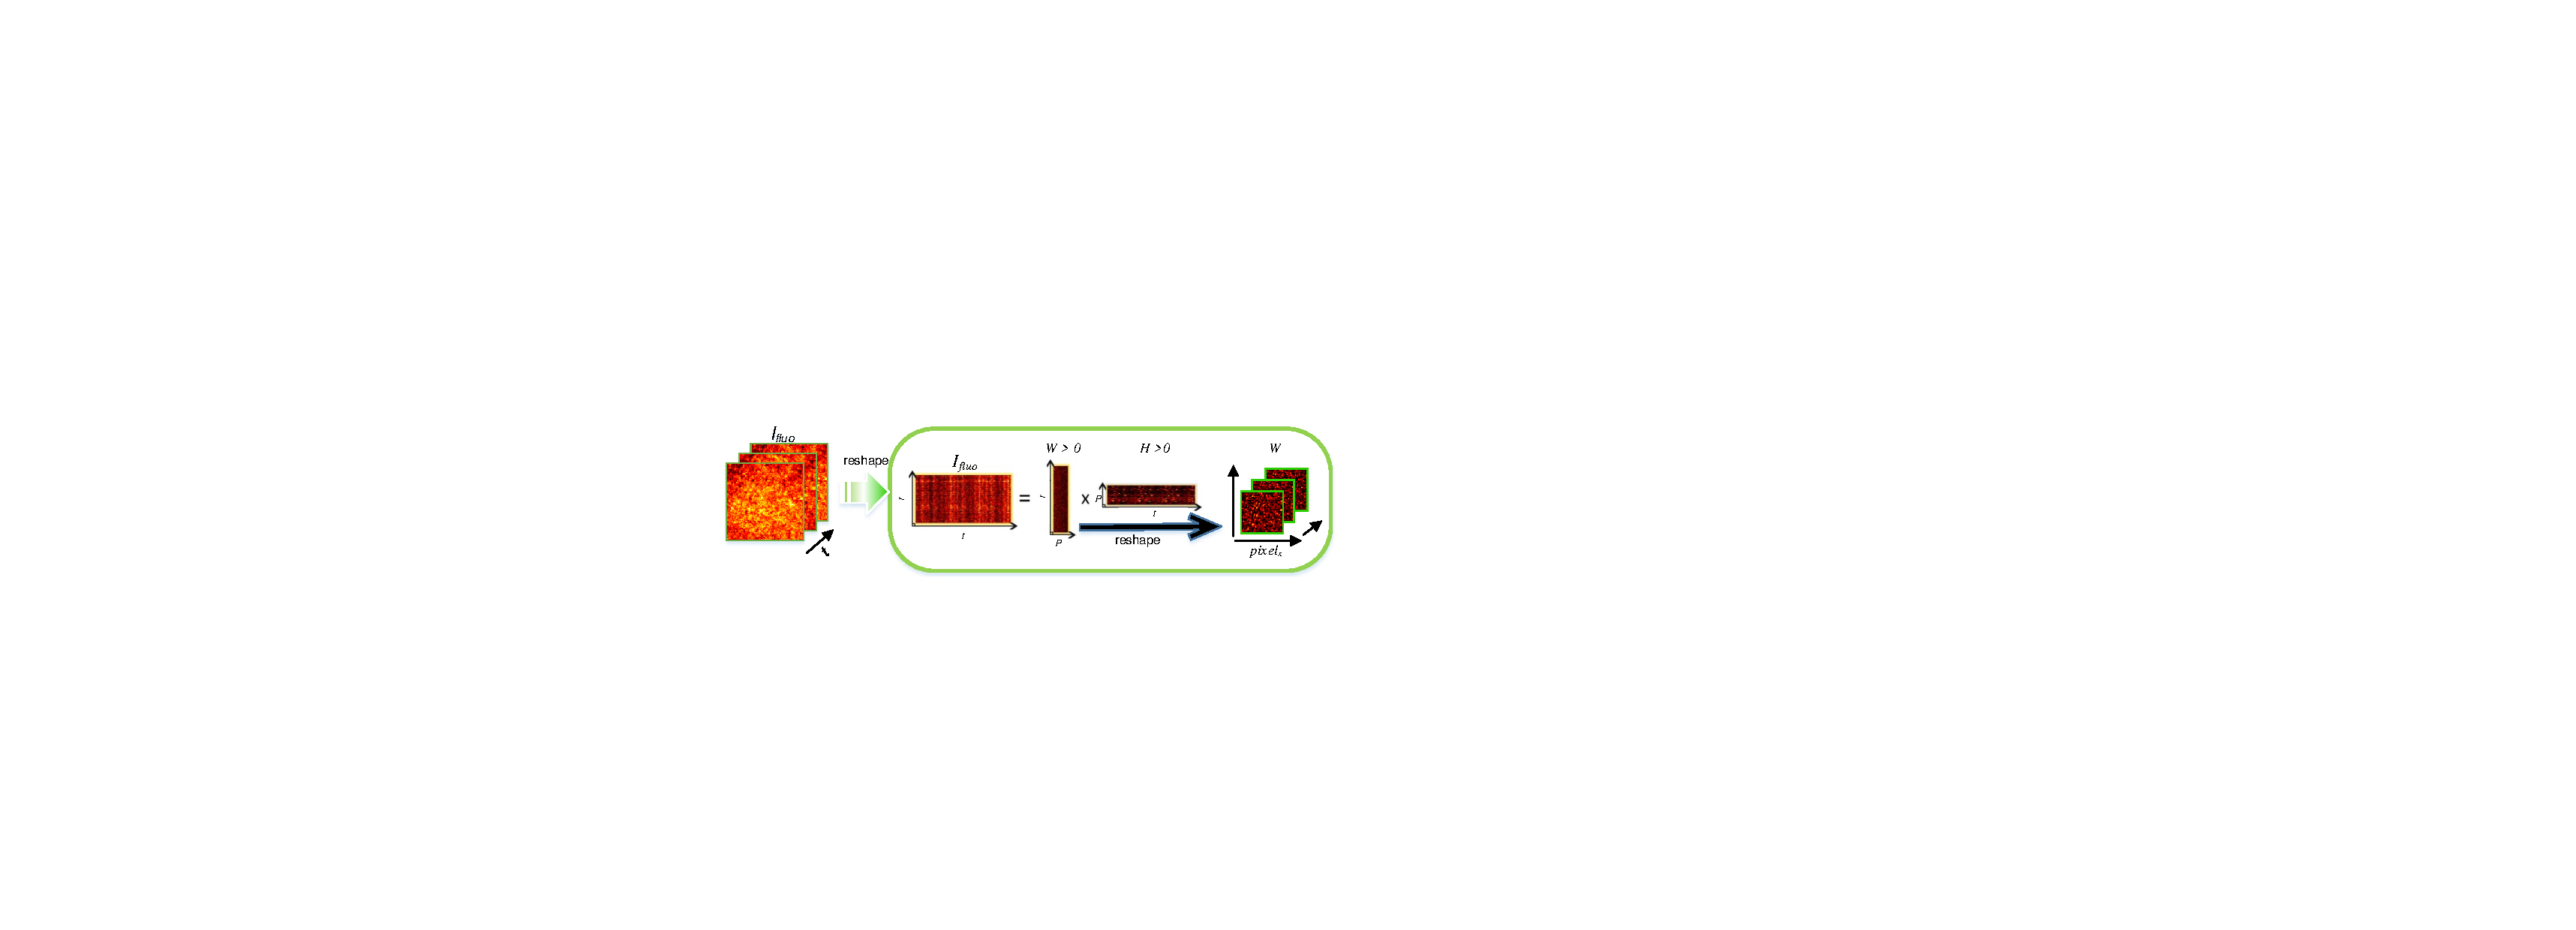
\includegraphics[scale=1.0]{C5.fig2}
	\caption{散斑指纹去混叠过程}
	\label{fig:5.2}
\end{figure}

\begin{figure}[htp]
	\centering
	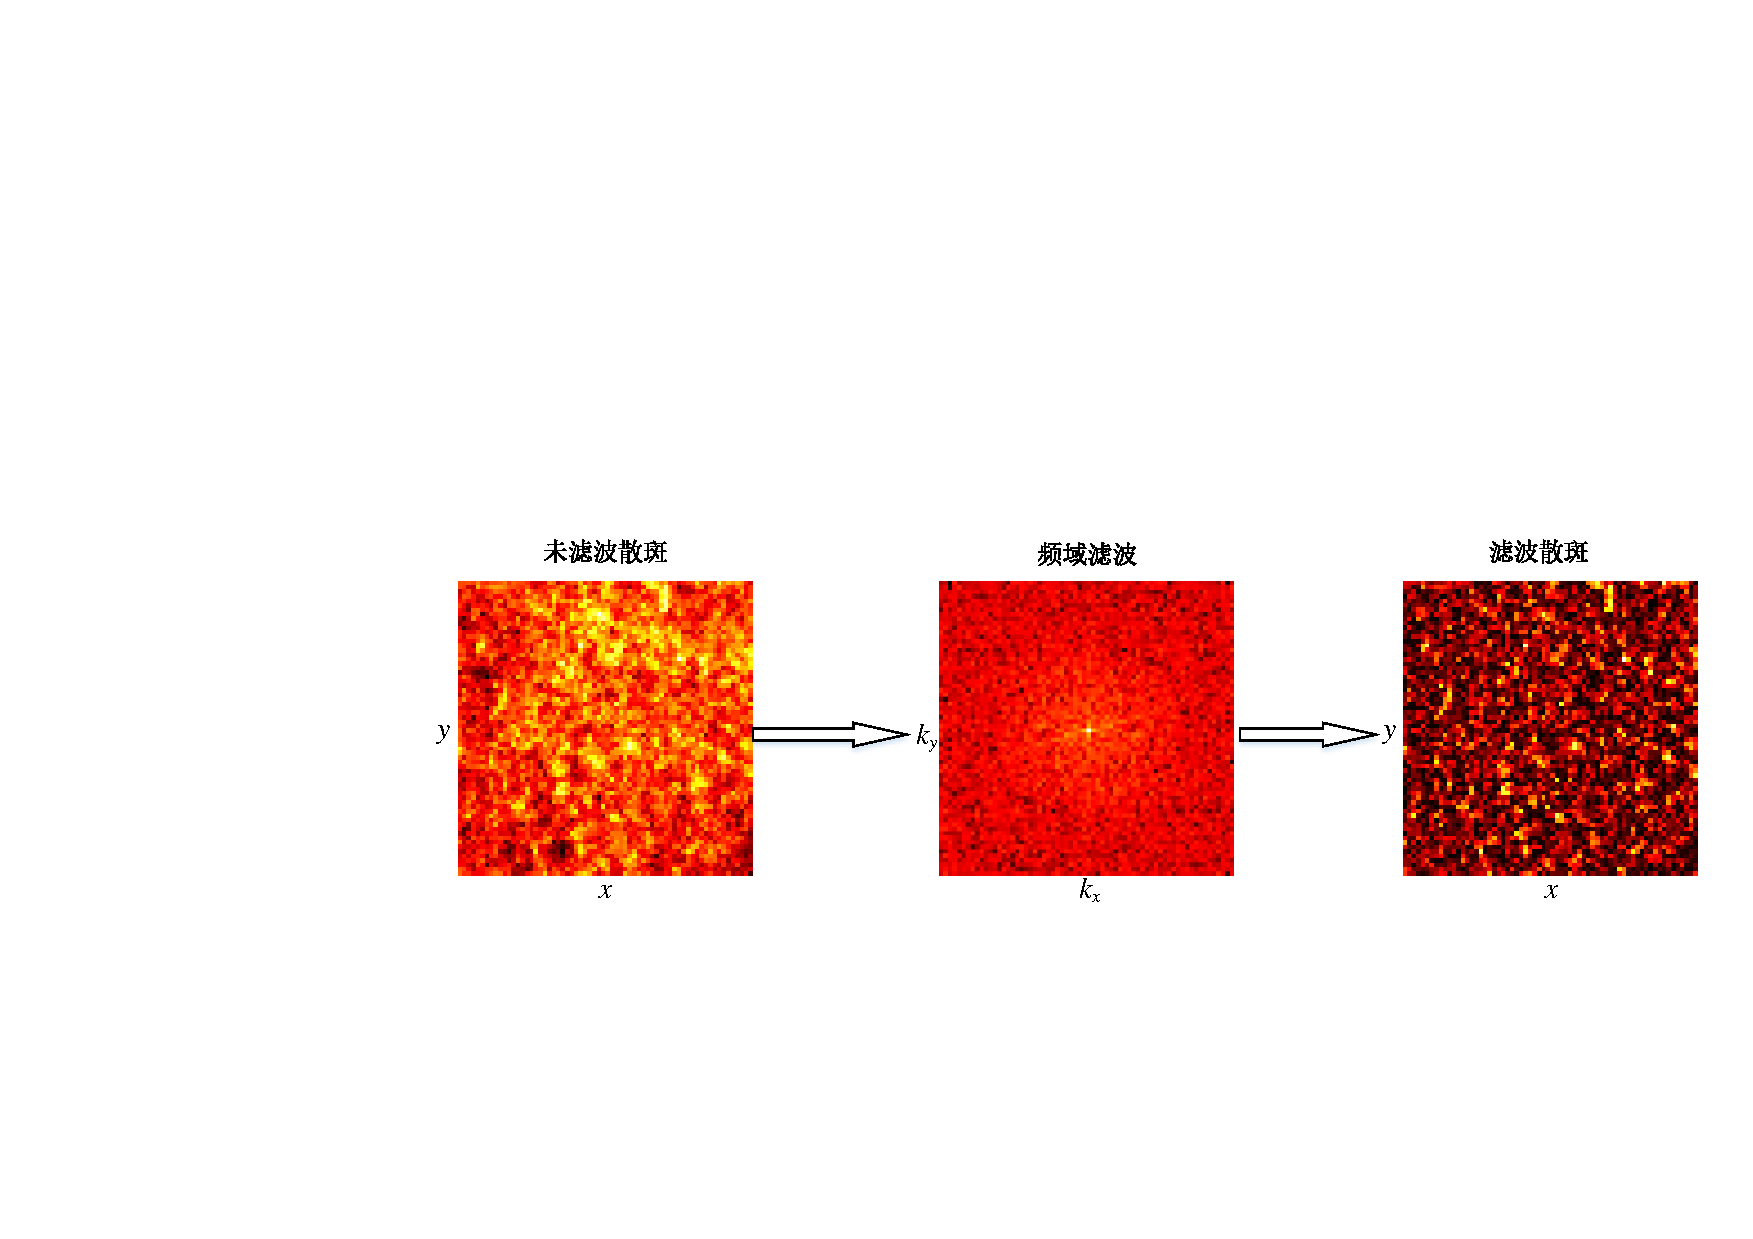
\includegraphics[scale=0.5]{C5.fig3}
	\caption{散斑滤波}
	\label{fig:5.3}
\end{figure}

为了运行NMF算法,矩阵秩$\rho$是唯一需要预先确定的参数。通常可以使用几种方法来估计$\rho$,例如使用 \textsl{k}-means 算法 \cite{Moretti2020a} 查看集群的数量,或者通过估计损失函数的“拐点”\cite{boniface_non_invasive_2020,hutchins_position_dependent_2008}。
在我们的使用情境下,为了简化该估计过程,我们尝试不同的数值作为该矩阵的$\rho$,记录不同数值所对应的均方根残差(Root Mean Square Residual,RMSR):$\vert\vert I_{fluo}-WH \vert\vert_{Fro}$。然后,RMSR最小值所对应的$\rho$,即该值为系统的秩$\rho$。为了验证我们所提出方法的有效性,于是进行了相应的仿真,仿真结果如图\ref{fig:5.5}所示。首先,我们生成5个点源目标,利用卷积模型生成各自的散斑指纹,并采用随机照明的方式对目标机型照明,记录其相应的散斑图案。然后根据前面所描述的矩阵秩$\rho$估计方法进行估计。图\ref{fig:5.5}中,三角形符号指示出RMSR的最小值,实线代表12次均方根值的平均值,每次的NMF优化采用不同的随机初始值。
三角形符号表示RMSR的最小均值,实线代表12次均方根值与NMF随机初始化值的均值,星号是误差条,表示其正负方向的标准偏差。通过仿真可知,当估计的秩$\rho$ 等于系统的真实秩$P$ 时,平均RMSR值为最小。我们同时分别尝试了,不同数量的点源目标,仿真结果如图\ref{fig:5.5}所示。其仿真结果表明:RMSR的最小值分别为:5,10和15,与真实值非常吻合。

\begin{figure}[htp]
	\centering
	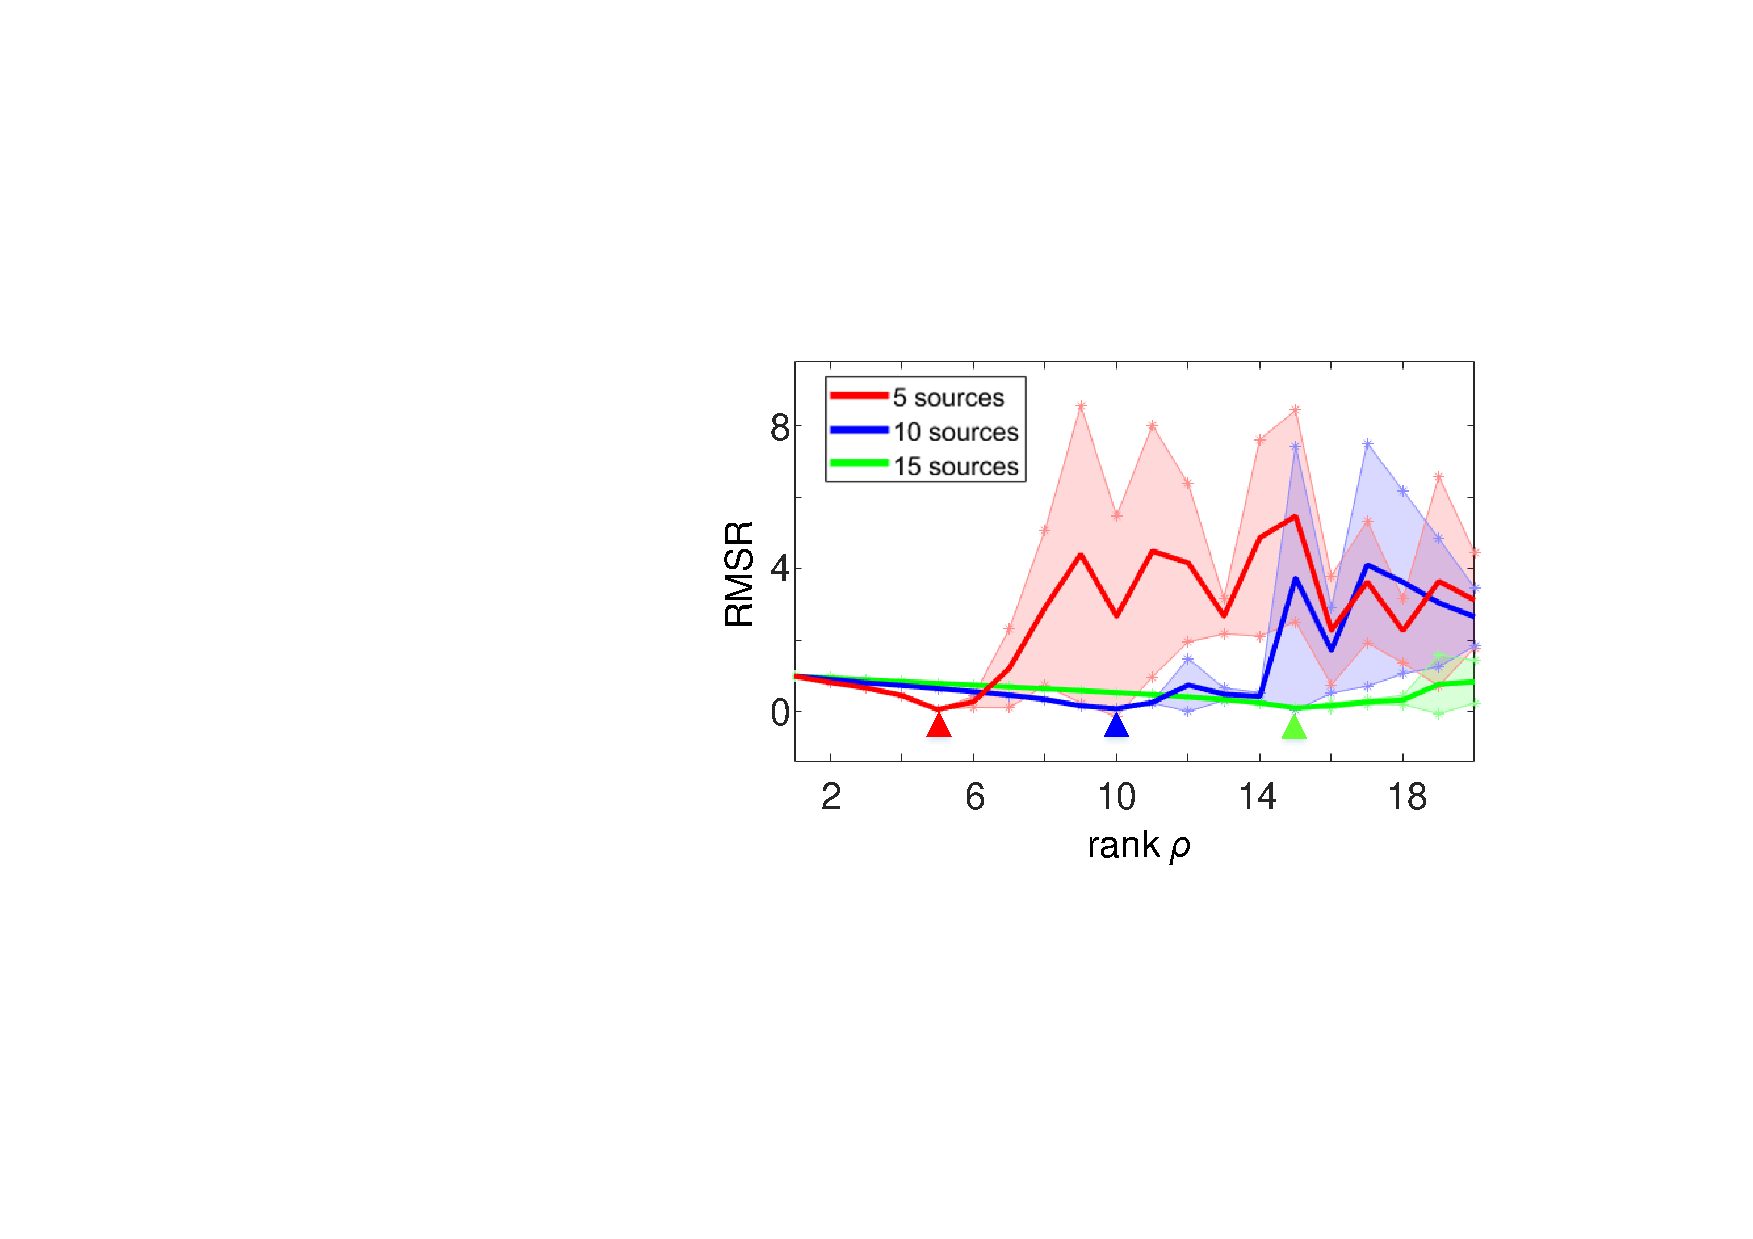
\includegraphics[scale=0.5]{C5.fig5}
	\caption{系统的秩$\rho$估计(仿真)}
	\label{fig:5.5}
\end{figure}

此外,我们通过实验证明该了估计方法的有效性。在实验中,通过随机放置11荧光珠为目标,利用旋转毛玻璃提供随机照明,记录其荧光散斑图案,并进行该数据集秩的估计,实验结果如图\ref{fig:5.6}所示。如图\ref{fig:5.6}(b)所示,所估计的$\rho$与系统真实$P$保持一致。同时,我们还在\ref{fig:5.6}(a)中提前展示了其图像的重建结果,左图为真实目标,右图为重建结果。通过仿真和实验的方式,证明了估计数据集秩的方法有效性。

\begin{figure}[htp]
	\centering
	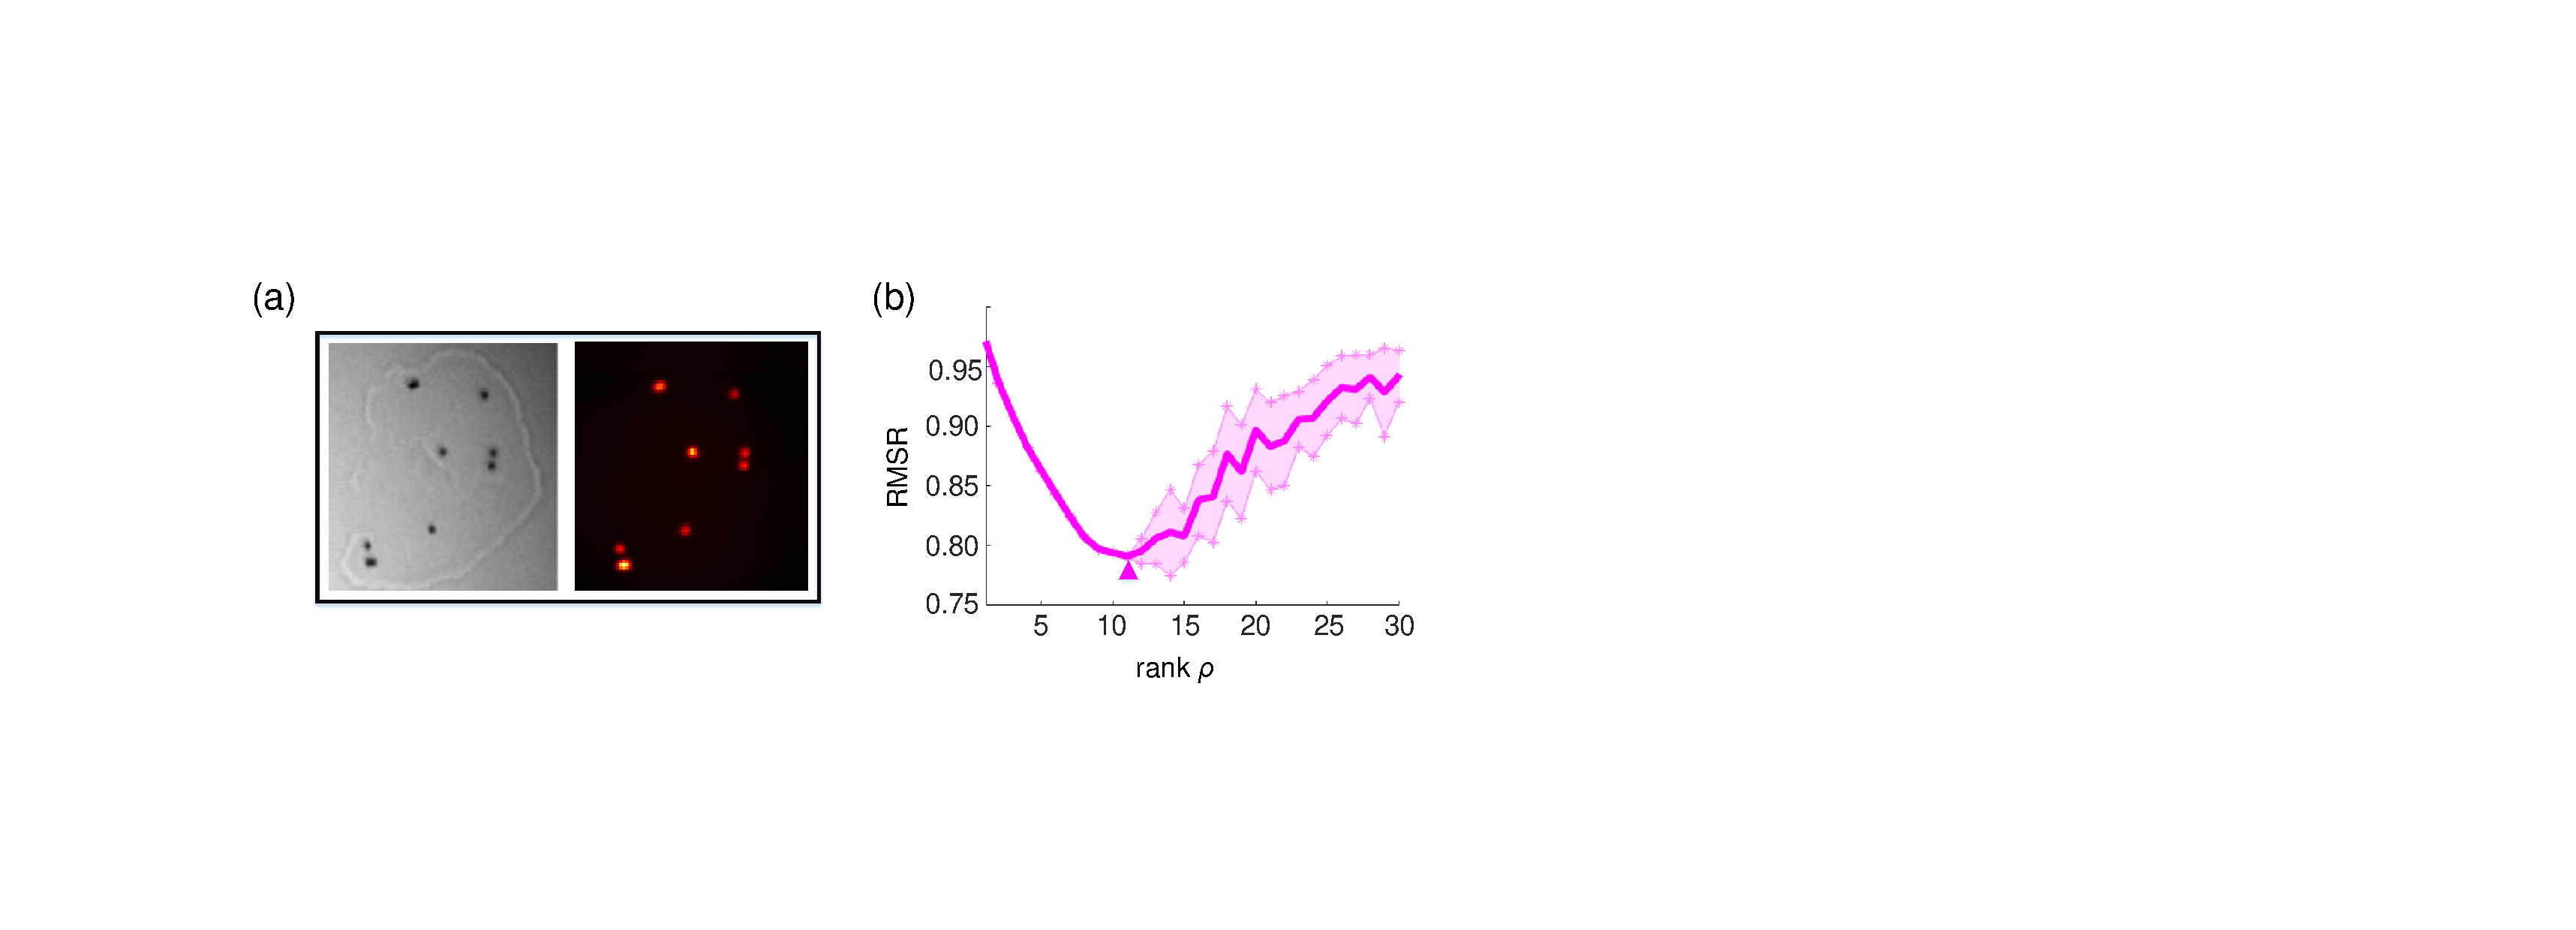
\includegraphics[scale=0.5]{C5.fig6}
	\caption{系统的秩$\rho$估计(实验)}
	\label{fig:5.6}
\end{figure}

\begin{figure}[htp]
	\centering
	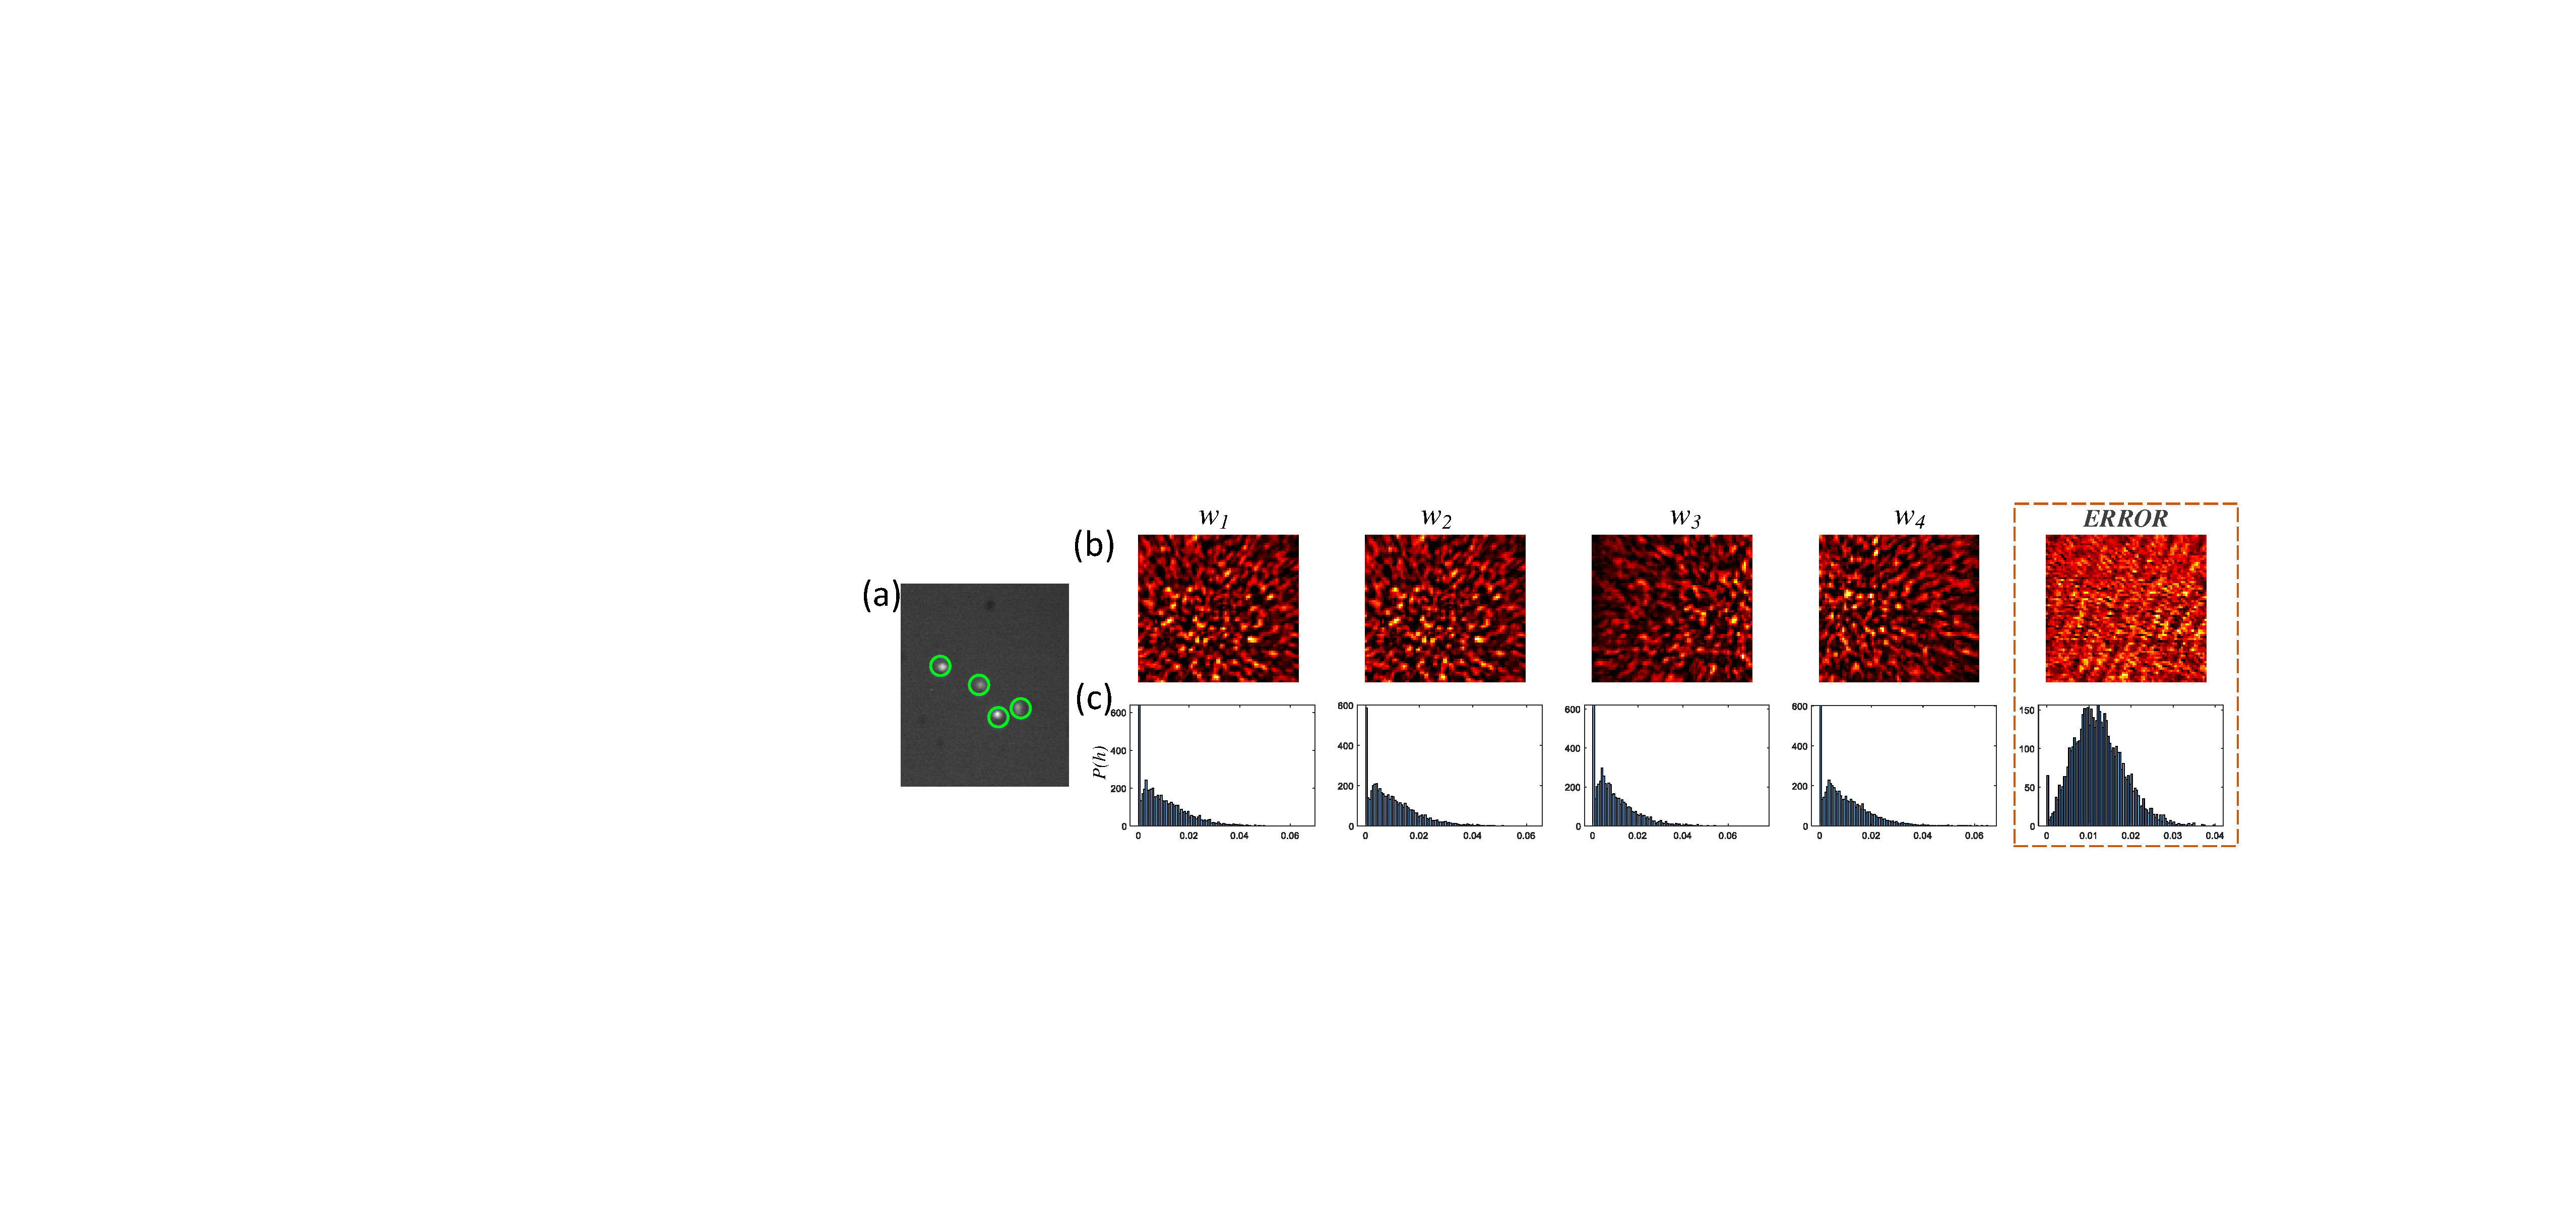
\includegraphics[scale=0.30]{C5.fig7}
	\caption{散斑去混叠实验结果}
	\label{fig:5.7}
\end{figure}

为了更加直观的显示散斑去混叠的结果,我们进行了另外一组实验,实验结果如图\ref{fig:5.7}所示。将一系列散斑图案$I$通过NMF算法,分解为矩阵$W$和$H$。图\ref{fig:5.7}(a)为原始目标,图\ref{fig:5.7}(b)为去混叠后散斑(来自于矩阵$W$)和图\ref{fig:5.7}(c)为对应图\ref{fig:5.7}(b)各自去混叠散斑的强度分布图,且属于瑞丽分布。如图\ref{fig:5.7}中,虚线所标出的去混叠散斑,该散斑为算法所制造的噪声,当没有正确的估计数据集的秩可能造成此种结果。可以通过分析去混叠散斑的强度分布图进行剔除操作。但是,在本章所提出的重建方法中未使用此操作。

\subsubsection*{\textbf{\textit{NMF算法}}}

NMF的早期工作是由芬兰的一组研究人员\cite{paatero_positive_1994}在1990年代中期以正矩阵分解的方式进行的。 在 Lee 和 Seung 之后,它被广泛称为非负矩阵分解研究了NMF的两种不同分解算法的特性\cite{lee_learning_1999,lee_algorithms_2001}。它们仅在量化近似质量的成本函数上略有不同。一种算法可以最小化传统的最小二乘误差,而另一种算法最小化广义Kullback-Leibler散度。在这里,我们仅描述在去混叠过程中所使用的的传统最小二乘误差类型。为了找到近似的因式分解$I \approx WH$,一个简单的评价函数为度量是 $I$ 和 $WH$ 之间的欧几里得距离的平方,即对应于Frobenius范数:

\begin{equation}
	\begin{aligned}
\Arrowvert I -WH\Arrowvert_F^{2} = \sum_{i,j} (I -WH)_{i,j}^2,
\label{eq:5.3}
\end{aligned}
\end{equation}

虽然函数$\Arrowvert I -WH\Arrowvert_F^{2}$仅在$W$或仅$H$是凸的,它的两个变量$W$和$H$不同时为凸。因此,通过寻找全局最小值去解决此问题较难实现。然而,有许多数值优化技术可用于寻找局部最小值。交替成本的最小化导致了交替最小二乘法 (Alternating Least Squares,ALS) 算法:在这种方法中,在$W$和$H$的初始随机初始化之后,迭代地执行 $W$ 固定 $H$ 和 执行$H$ 固定 $W$ 的最小二乘解,直到成本函数达到最小值,或连续迭代之间的成本函数差异变得小于给定的容差值,或达到最大迭代次数。在每次迭代中,$W$和$H$ 的负元素被替换为$0$或很小的数。由于NMF算的稳定性和可解释性,该算法已经在众多领域有着较多的应用。

\subsection{基于散斑指纹的图像重建}

当进行散斑去混叠步骤后,每个独立点光源的的散斑指纹被获取。由于OME\cite{Freund1988,katz_non-invasive_2014,bertolotti_non-invasive_2012}可知,当两个位于散射介质后的独立点光源属于同一个OME范围时,两个点光源据所产生的散斑变现为相互之间的平移,其位移距离等于他们的相对距离。如:两个点光源之间的距离$\delta u$和散斑之间的平移距离为$\delta v$,根据OME我们可知:$\delta v = M \cdot \delta u$,其中$M$为光学系统的放大率,如图\ref{fig:5.8}所示。当成像系统中存在OME,利用去混叠方法分别获取来自不同点光源的散斑指纹,然后探索散斑指纹之间的共享信息来重建隐藏目标。
在图\ref{fig:5.8}中,$\delta u$为两个点源目标之间的距离,$\# 1$和$\# 2$分别表示点源目标$\# 1$和$\# 2$,将点源$\# 1$的散斑指纹看作参考散斑,分别计算散斑指纹$\# 1$和$\# 1$,$\# 1$和$\# 2$的互相关。
散斑指纹$\# 1$和$\# 1$的互相关信息会产生一个$\delta $位于图像中心,散斑指纹$\# 1$和$\# 2$的互相关信息会产生一个$\delta $距离中心为$\delta v$的图像。
从图\ref{fig:5.8}可以看出,通过计算散斑之间的互相关可以获取对应点源目标的相对位置。在此,不同点源目标之间的相对位置信息可以被获取,如图\ref{fig:5.8}所恢复的信息更接近与点源目标的定位,仍然缺少图像信息。

\begin{figure}[htp]
	\centering
	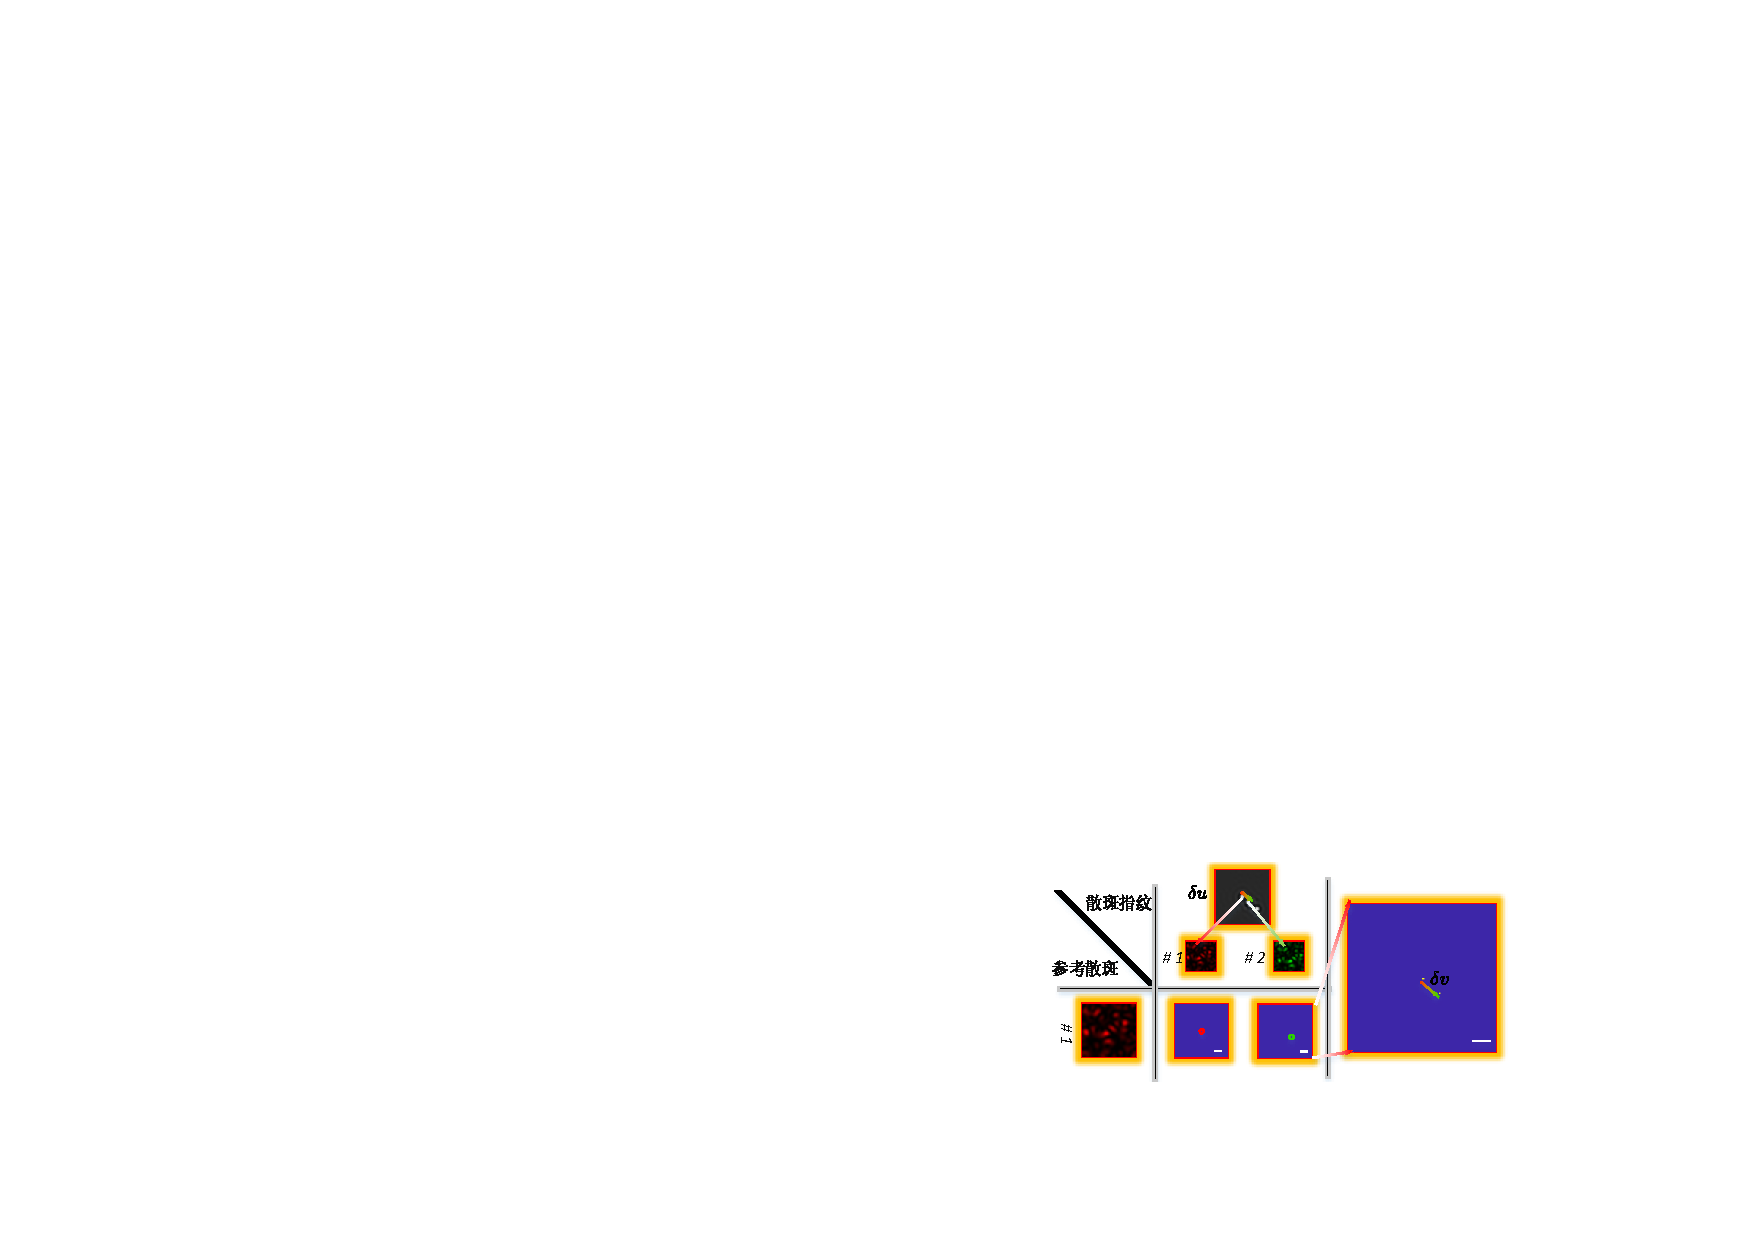
\includegraphics[scale=1.5]{C5.fig8}
	\caption{散斑的相关性探索}
	\label{fig:5.8}
\end{figure}

当获得不同点源目标的散斑指纹后,我们是否可以通过去卷积的方式实现图像重建呢?将某个散斑作为系统的PSF,然后进行去卷积运算\cite{biggs_acceleration_1997}。去卷积运算后,能获得该散斑图案对应于PSF时所产生的图案,不同散斑指纹之间的去卷积结构如图\ref{fig:5.9}所示。图\ref{fig:5.9}(a)为不同的散斑指纹和系统参考散斑(PSF),不同散斑指纹与PSF之间去卷积后的图像$I_{i}$。图\ref{fig:5.9}(b)为所有去卷积后图像$I_{i}$的加和图案$\sum_{i}^{n} I_{i}$,图\ref{fig:5.9}(c)为$\sum_{i}^{2} I_{i}$的加和,图\ref{fig:5.9}(d)为原始目标。从图\ref{fig:5.9}所示的结果可知,所有散斑指纹与参考散斑进行去卷积运算,并将去卷积后的结果进行加单的加和,可以获得图像\ref{fig:5.9}(b)。此时所获得重建结果\ref{fig:5.9}(b)与原始图像\ref{fig:5.9}(d)高度吻合,图\ref{fig:5.9}所示的目标均位于同一个OME范围内。

\begin{figure}[htp]
	\centering
	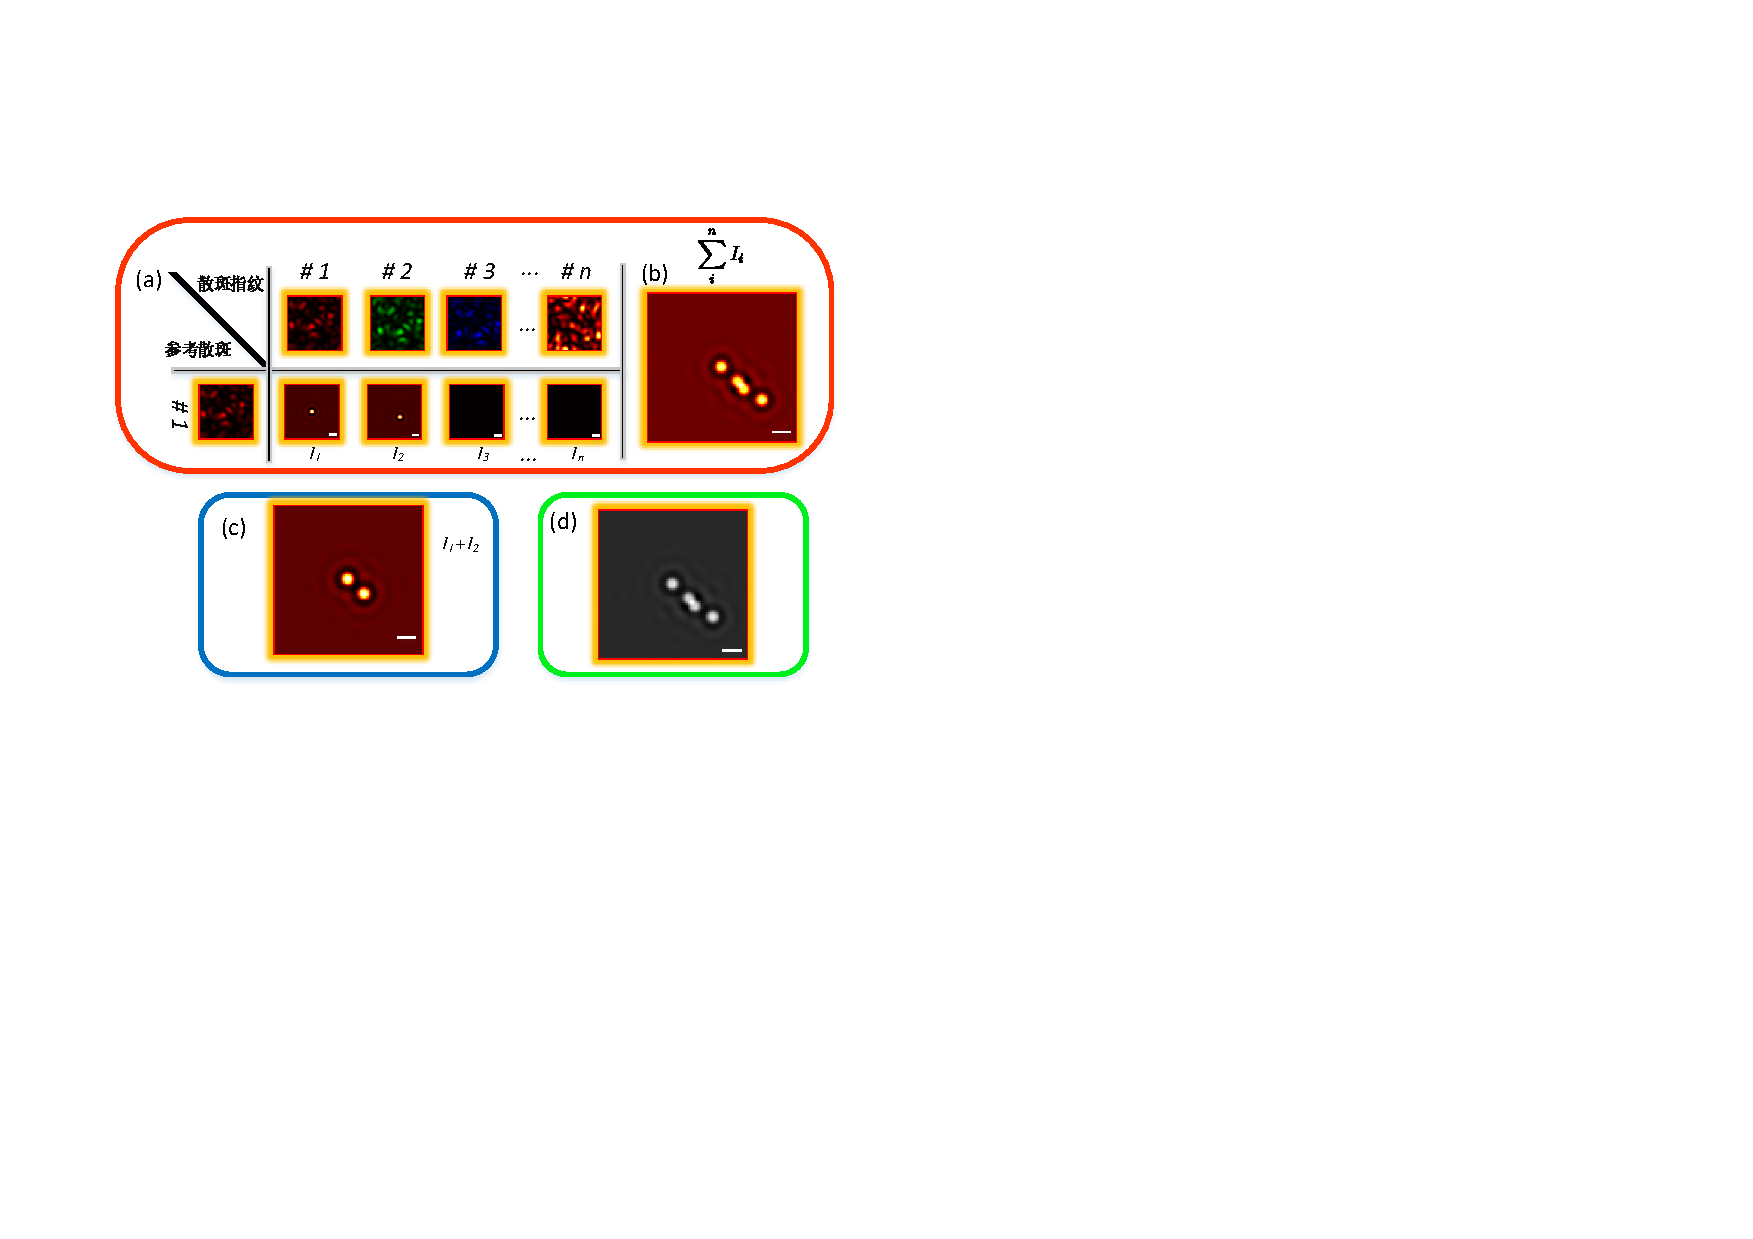
\includegraphics[scale=1.0]{C5.fig9}
	\caption{去卷积结果(OME范围内)}
	\label{fig:5.9}
\end{figure}

受到图\ref{fig:5.9}所示结果的启发,我们提出了本章的核心重建算法-基于散斑指纹的图像重建。无论两个点光源是否位同一个OME内,都可以通过 $k$\textsl{-th} 点光源对 $i$\textsl{-th} 点光源进行成对反卷积,可以写为:

\begin{equation}
	\begin{aligned}
\underset{o_{i,k}}{\arg\min \;\;}
\frac{\mu}{2} \vert\vert w_{i}-o_{i,k}* w_{k}\vert\vert^2_{2}+\vert\vert o_{i,k}\vert\vert_{TV}
\label{eq:5.4}
\end{aligned}
\end{equation}
其中$\mu$是正则化参数,$*$表示卷积算子,$\vert\vert \mathbf{f}\vert\vert_2 = \sqrt{\sum_{i} \vert f_i\vert^2} $表示$L_{2}$向量范数,
$\vert\vert \mathbf{f} \vert\vert_{TV} = \sum_{i}\sqrt{[D_x\mathbf{f}]_i^2 +[D_y\mathbf{f}]_i^2}$ 表示总变差 (Total variation,TV) 范数($D_x$ 和 $D_y$ 是沿水平和垂直方向的前向有限差分算子)。
这两个指纹被表示为$w_{i}$(被认为是“图像”)和$w_{k}$(被认为是“点扩散函数”,即PSF)。当两个点光源位于同一OME范围内时,成对反卷积会产生一个具有窄 $\delta$ 类峰值的均匀图像,该图像位于与两个点光源的相对位置($\vec{r} _{i,k} = \vec{r}_i - \vec{r}_k$)。如果两个点光源位于OME范围之外,则反卷积会产生噪声。

对于给定的点光源$k$,只需将与该点光源相关的所有成对反卷积的结果相加,就可以获得点光源附近物体的局部图像$o_{i,k}$。

\begin{equation}
		\begin{aligned}
O_{k} = \sum^{\rho}_{i=1}
o_{i,k}
\label{eq:5.5}
\end{aligned}
\end{equation}

即使点光源的集合扩展到远远超出OME范围,如果不同的等平面斑块由点光源“连接”,则可以恢复完整的空间分布。例如,如果点光源$i$和$k$超出OME范围但点光源$j$在它们之间,我们总是可以将它们之间的偏移计算为 $\vec{r_{i,k}} = \vec {r_{i,j}} + \vec{r_{j,k}}$。全局重建 $O^{Global}$ 可以通过将所有局部图像 $O_{k}$ 组合成一个图像来获得,同时考虑到它们相对于第一个点光源的相对位置 $\vec{r_{k,1}}$ :
\begin{equation}
	\begin{aligned}
O^{Global} = \sum^{\rho}_{k=1}
O_{k}(\vec{r} - \vec{r_{k,1}})
\label{eq:5.6}
\end{aligned}
\end{equation}

在去卷积过程中,不同的去卷积算法将会产生不同的重建结果,不同去卷积方法之间的对比将会在后续部分进行展示。在后续部分,基于散斑指纹的图像重建(Fingerprint-based reconstruction)简化为FBR。

\section{实验验证}

上面部分,我们对基本原理和图像重建方法进行阐述,接下来对实验部分进行描述。实验装置如图\ref{fig:5.11}所示,连续激光器($\lambda  = 532 nm $,Coherent Sapphire)的输出光经准扩束准直后,照射至旋转全息散射介质 (Edmund,DG10)。经过旋转全息散射介质调制后的光通过焦距为$200 mm$透镜(LA1708-A,Thorlabs)和物镜(Zeiss W “Plan-Apochromat” $\times 20$,NA $1.0$),并照明荧光目标。荧光目标被激光击发后产生荧光信号,荧光信号反向传播通过物镜(Zeiss W “Plan-Apochromat” $\times 20$,NA $1.0$)和焦距为$200 mm$的镜筒透镜(L,AC254-150-A,Thorlabs),被sCMOS探测器(Hamamatsu ORCA Flash)接收。两个二向色滤光片(MF525-39,Thorlabs)用于屏蔽除荧光信号以外的信号。其中,RD:旋转散射介质,DM:二向色散镜,OB 1(OB 2):物镜,Scat.:散射介质,Object:目标,SF:光谱滤波片,TL 1(TL 2):镜筒透镜。

\begin{figure}[htp]
	\centering
	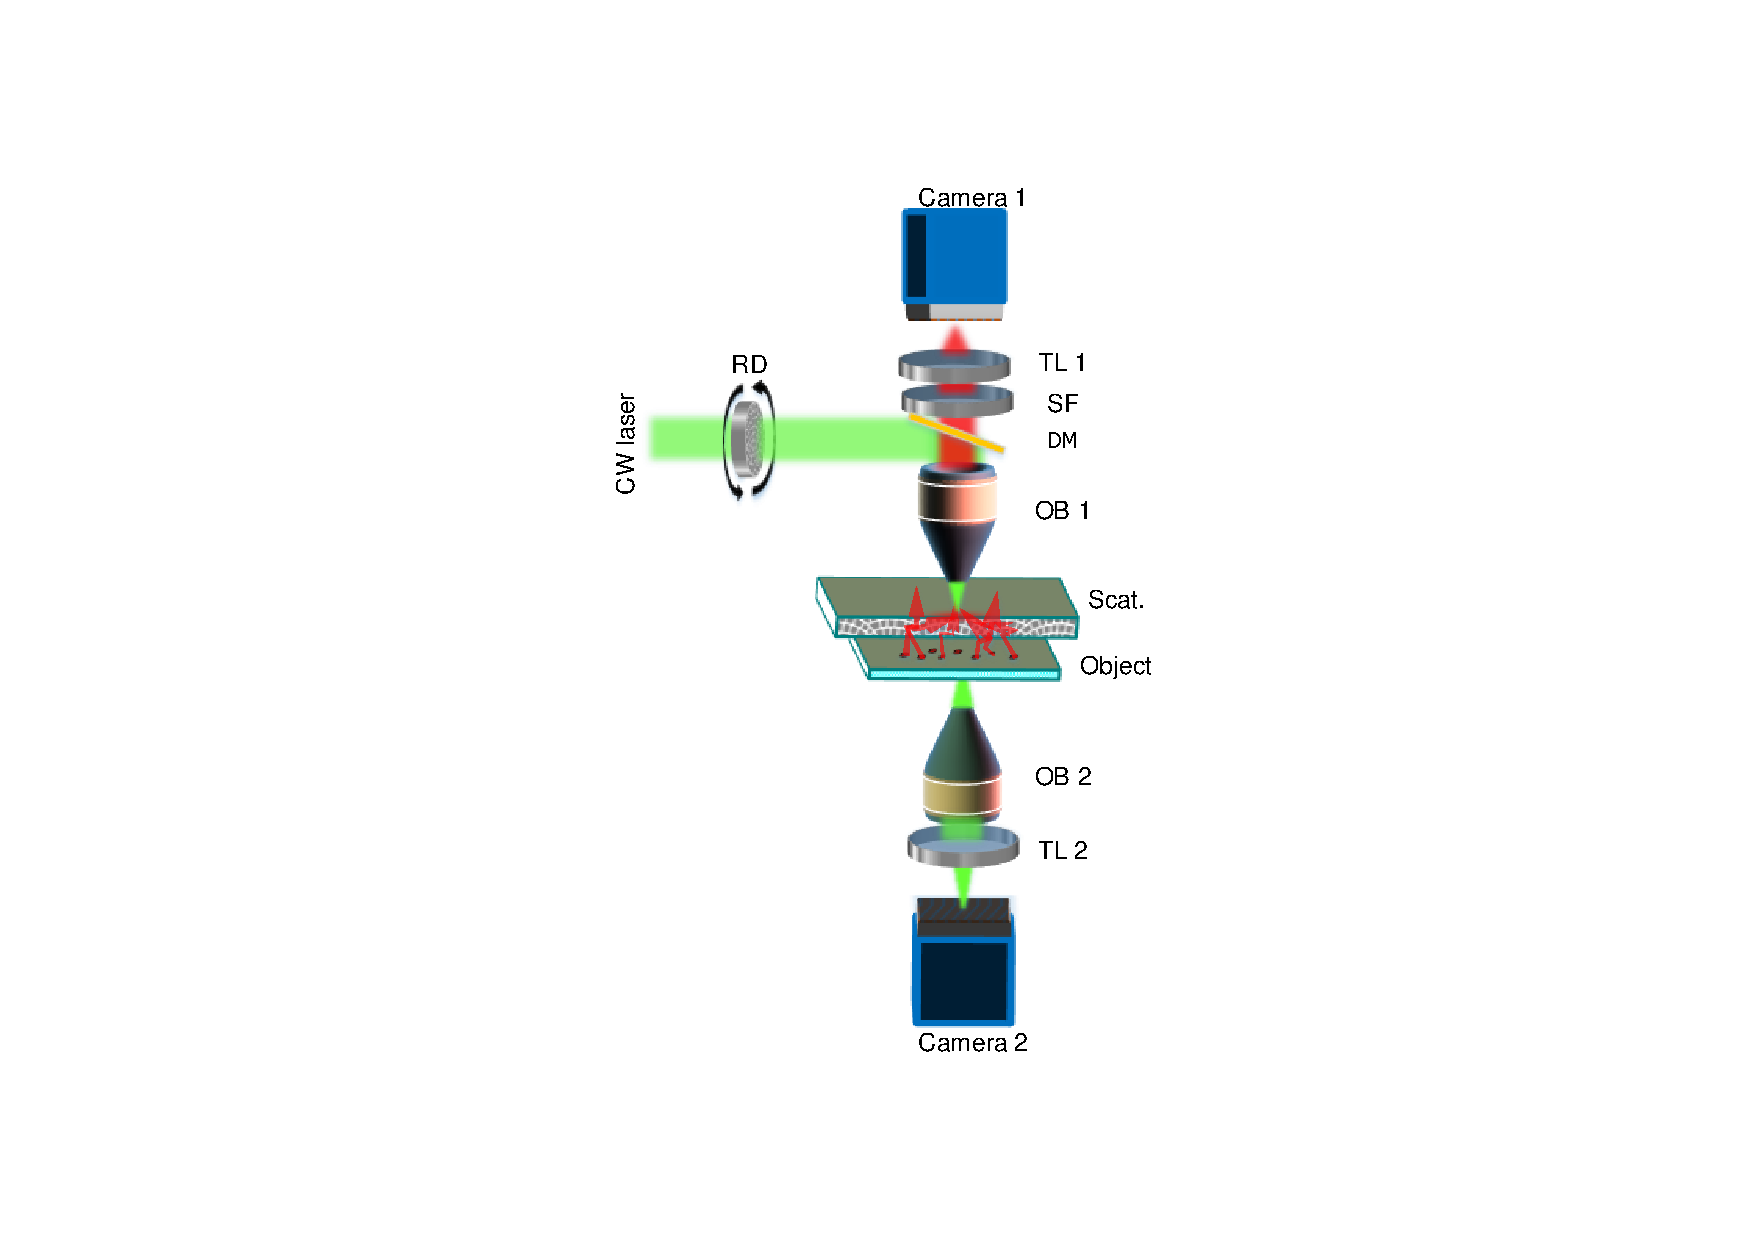
\includegraphics[scale=0.7]{C5.fig11}
	\caption{实验装置示意图}
	\label{fig:5.11}
\end{figure}

\begin{figure}[htp]
	\centering
	
\includegraphics[scale=0.41]{C5.fig12}
	\caption{基于波动随机照明的透过散射介质超OME范围成像流程示意图}
	\label{fig:5.12}
\end{figure}

实验中,荧光物体由橙色荧光珠($540/560 nm$,Invitrogen FluoSpheres,size $1.0 um$)和花粉种子形状的荧光目标(Carolina, Mixed Pollen Grains Slide, $wm$)组成。荧光目标放置于散射介质下方,散射介质与荧光物体的距离为$0.2 mm$。在实验中,我们拥有控制部分,此部分仅用于检测是否正确防止目标。该部分由显微镜物镜(Olympus 'MPlan N' $\times 20$, NA $0.4$)、$ 150 mm$ 镜筒透镜(L, AC254-150-A,Thorlabs)和CCD相机(Allied Vision,Manta)组成。白色光源(Moritex,MHAB 150W)为该部分提供照明,帮助正确选择荧光物体的位置,它还允许我们对实验装置进行对其校准。
\subsection{稀疏2D荧光目标重建}
我们利用上面说介绍过的橙色荧光珠作为2D目标,进行了基于随机照明的大视场超OME成像实验,实验流程和结果如图\ref{fig:5.12}所示。在图\ref{fig:5.12}(a)中,相干光源照亮旋转全息散射介质,利用散射介质随机调制散斑图案来激发荧光物体。 荧光物体一旦被激发,荧光物体发出的信号就会被相机记录下来。 $I_{fluo}$ 是一系列 $t$ 荧光散斑,对应于不同的随机散斑照明,散斑指纹可以通过使用NMF从 $I_{fluo}$ 中恢复。图\ref{fig:5.12}(b-e)为图像重建过程,(b)在所有可能的散斑指纹对之间执进行成对反卷积(标记为 $*^{-1}$)。(c)每个反卷积的结果提供了一个点光源与其相邻点光源之间的相对位置。(d) 通加所有散斑指纹和特定散斑指纹的去卷积结果,可以恢复以该散斑指纹对应的点光源为中心的对象的局部图像(参见公式\ref{eq:5.5})。(e) 根据相邻点光源之间的相对位置,可以将所有部分图像合并到最终全局重建。虚线圆圈表示光学记忆范围。比例尺大小为 $10 um$。RD:旋转扩散器,DM:二向色镜,OB:物镜,Scat.:散射介质,Fluo。 Obj.:荧光物体,SF:光谱滤波器,TL:镜筒透镜。同时为更加详细的展示重建的局部图像,我们将图\ref{fig:5.12}(d)所对应的所有图像进行详尽展示,如图\ref{fig:5.10}所示。

\begin{figure}[htp]
	\centering
	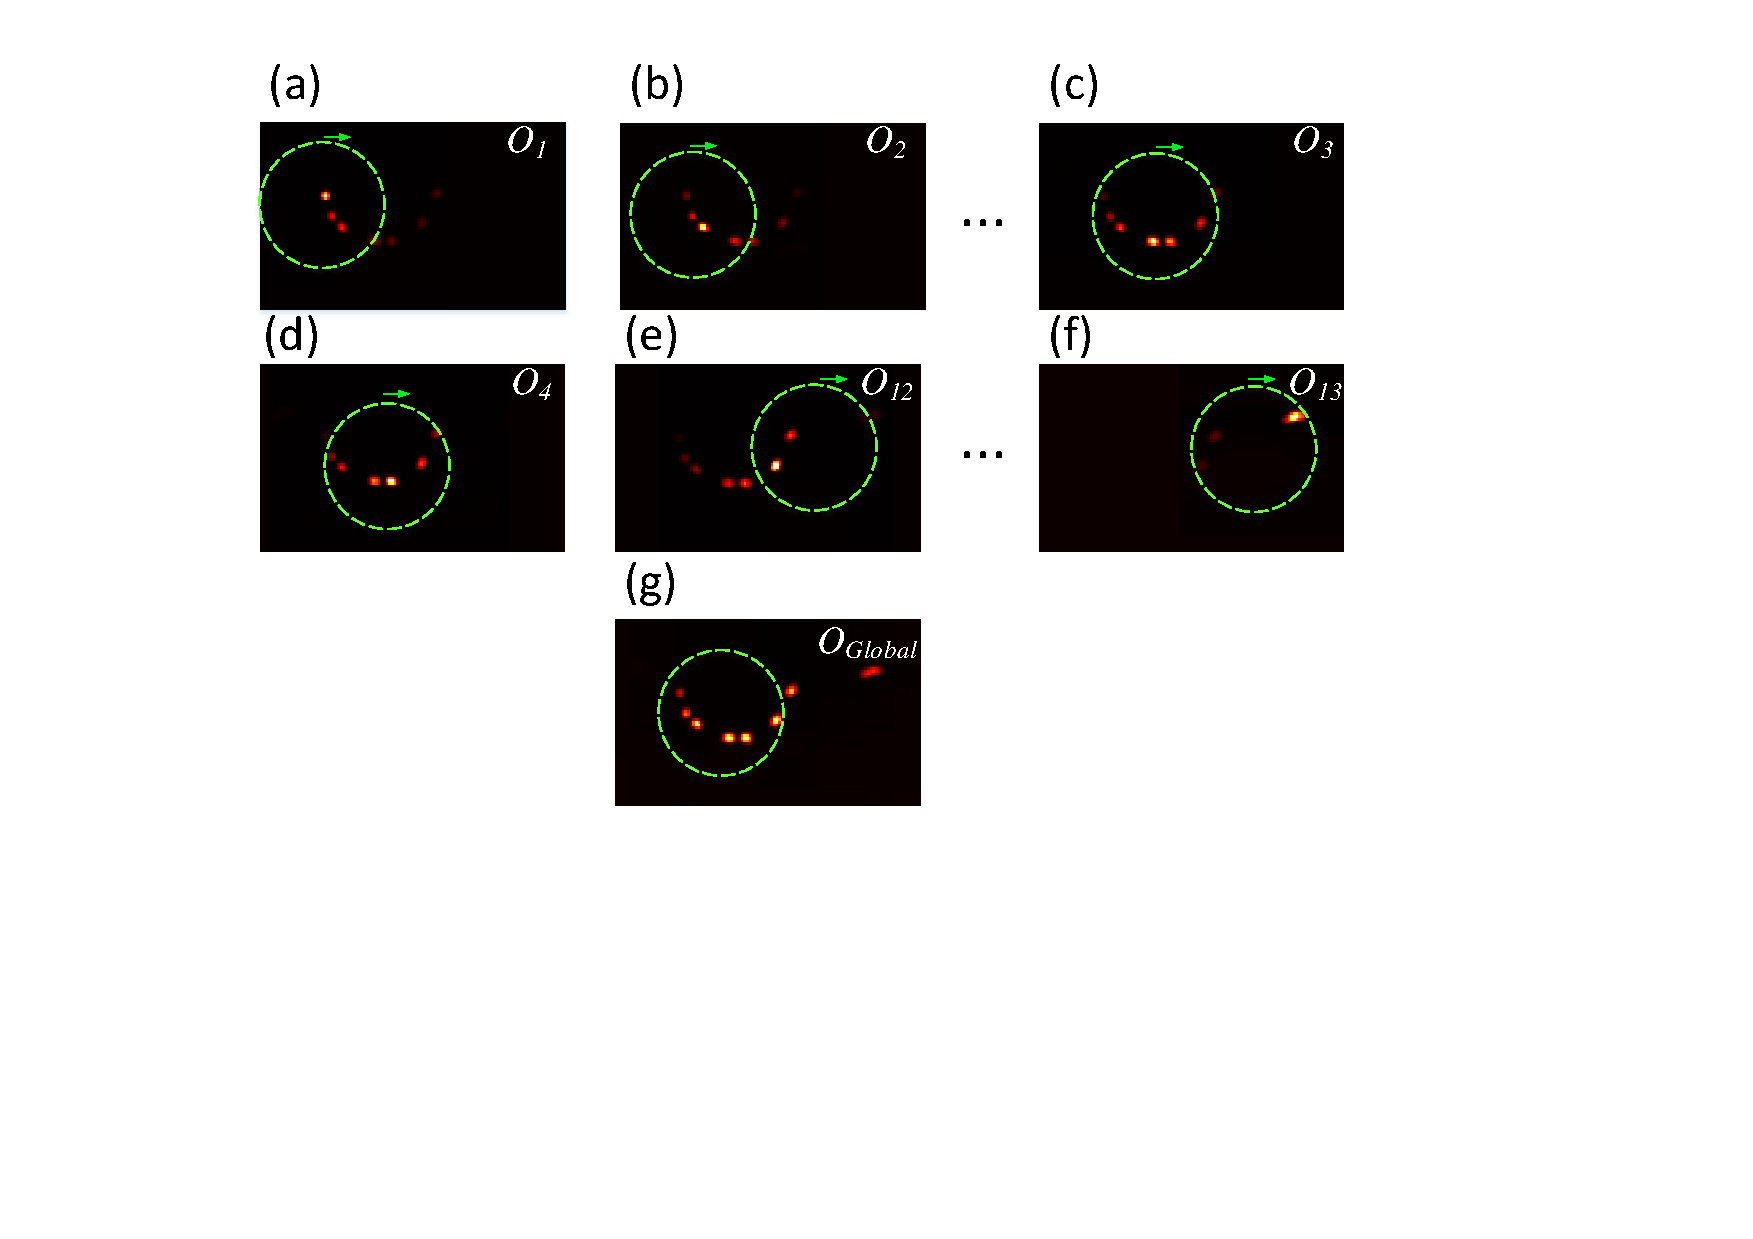
\includegraphics[scale=0.7]{C5.fig10}
	\caption{FBR重建流程}
	\label{fig:5.10}
\end{figure}

图\ref{fig:5.10}(a)-(f)为选择不同的散斑指纹为PSF,进行去卷积运算所获得局部图像$O_{k}$,图\ref{fig:5.10}(g)为全局重建图像,图\ref{fig:5.10}所示的结果采用的去卷积方法来自于参考文献\cite{Chan2011}。其中,RD:旋转散射介质,DM:二向色散镜,OB:物镜,Scat.:散射介质,Fluo. Obj.:荧光目标,SF:光谱滤波片,TL:管透镜。

\begin{figure}[htp]
	\centering
	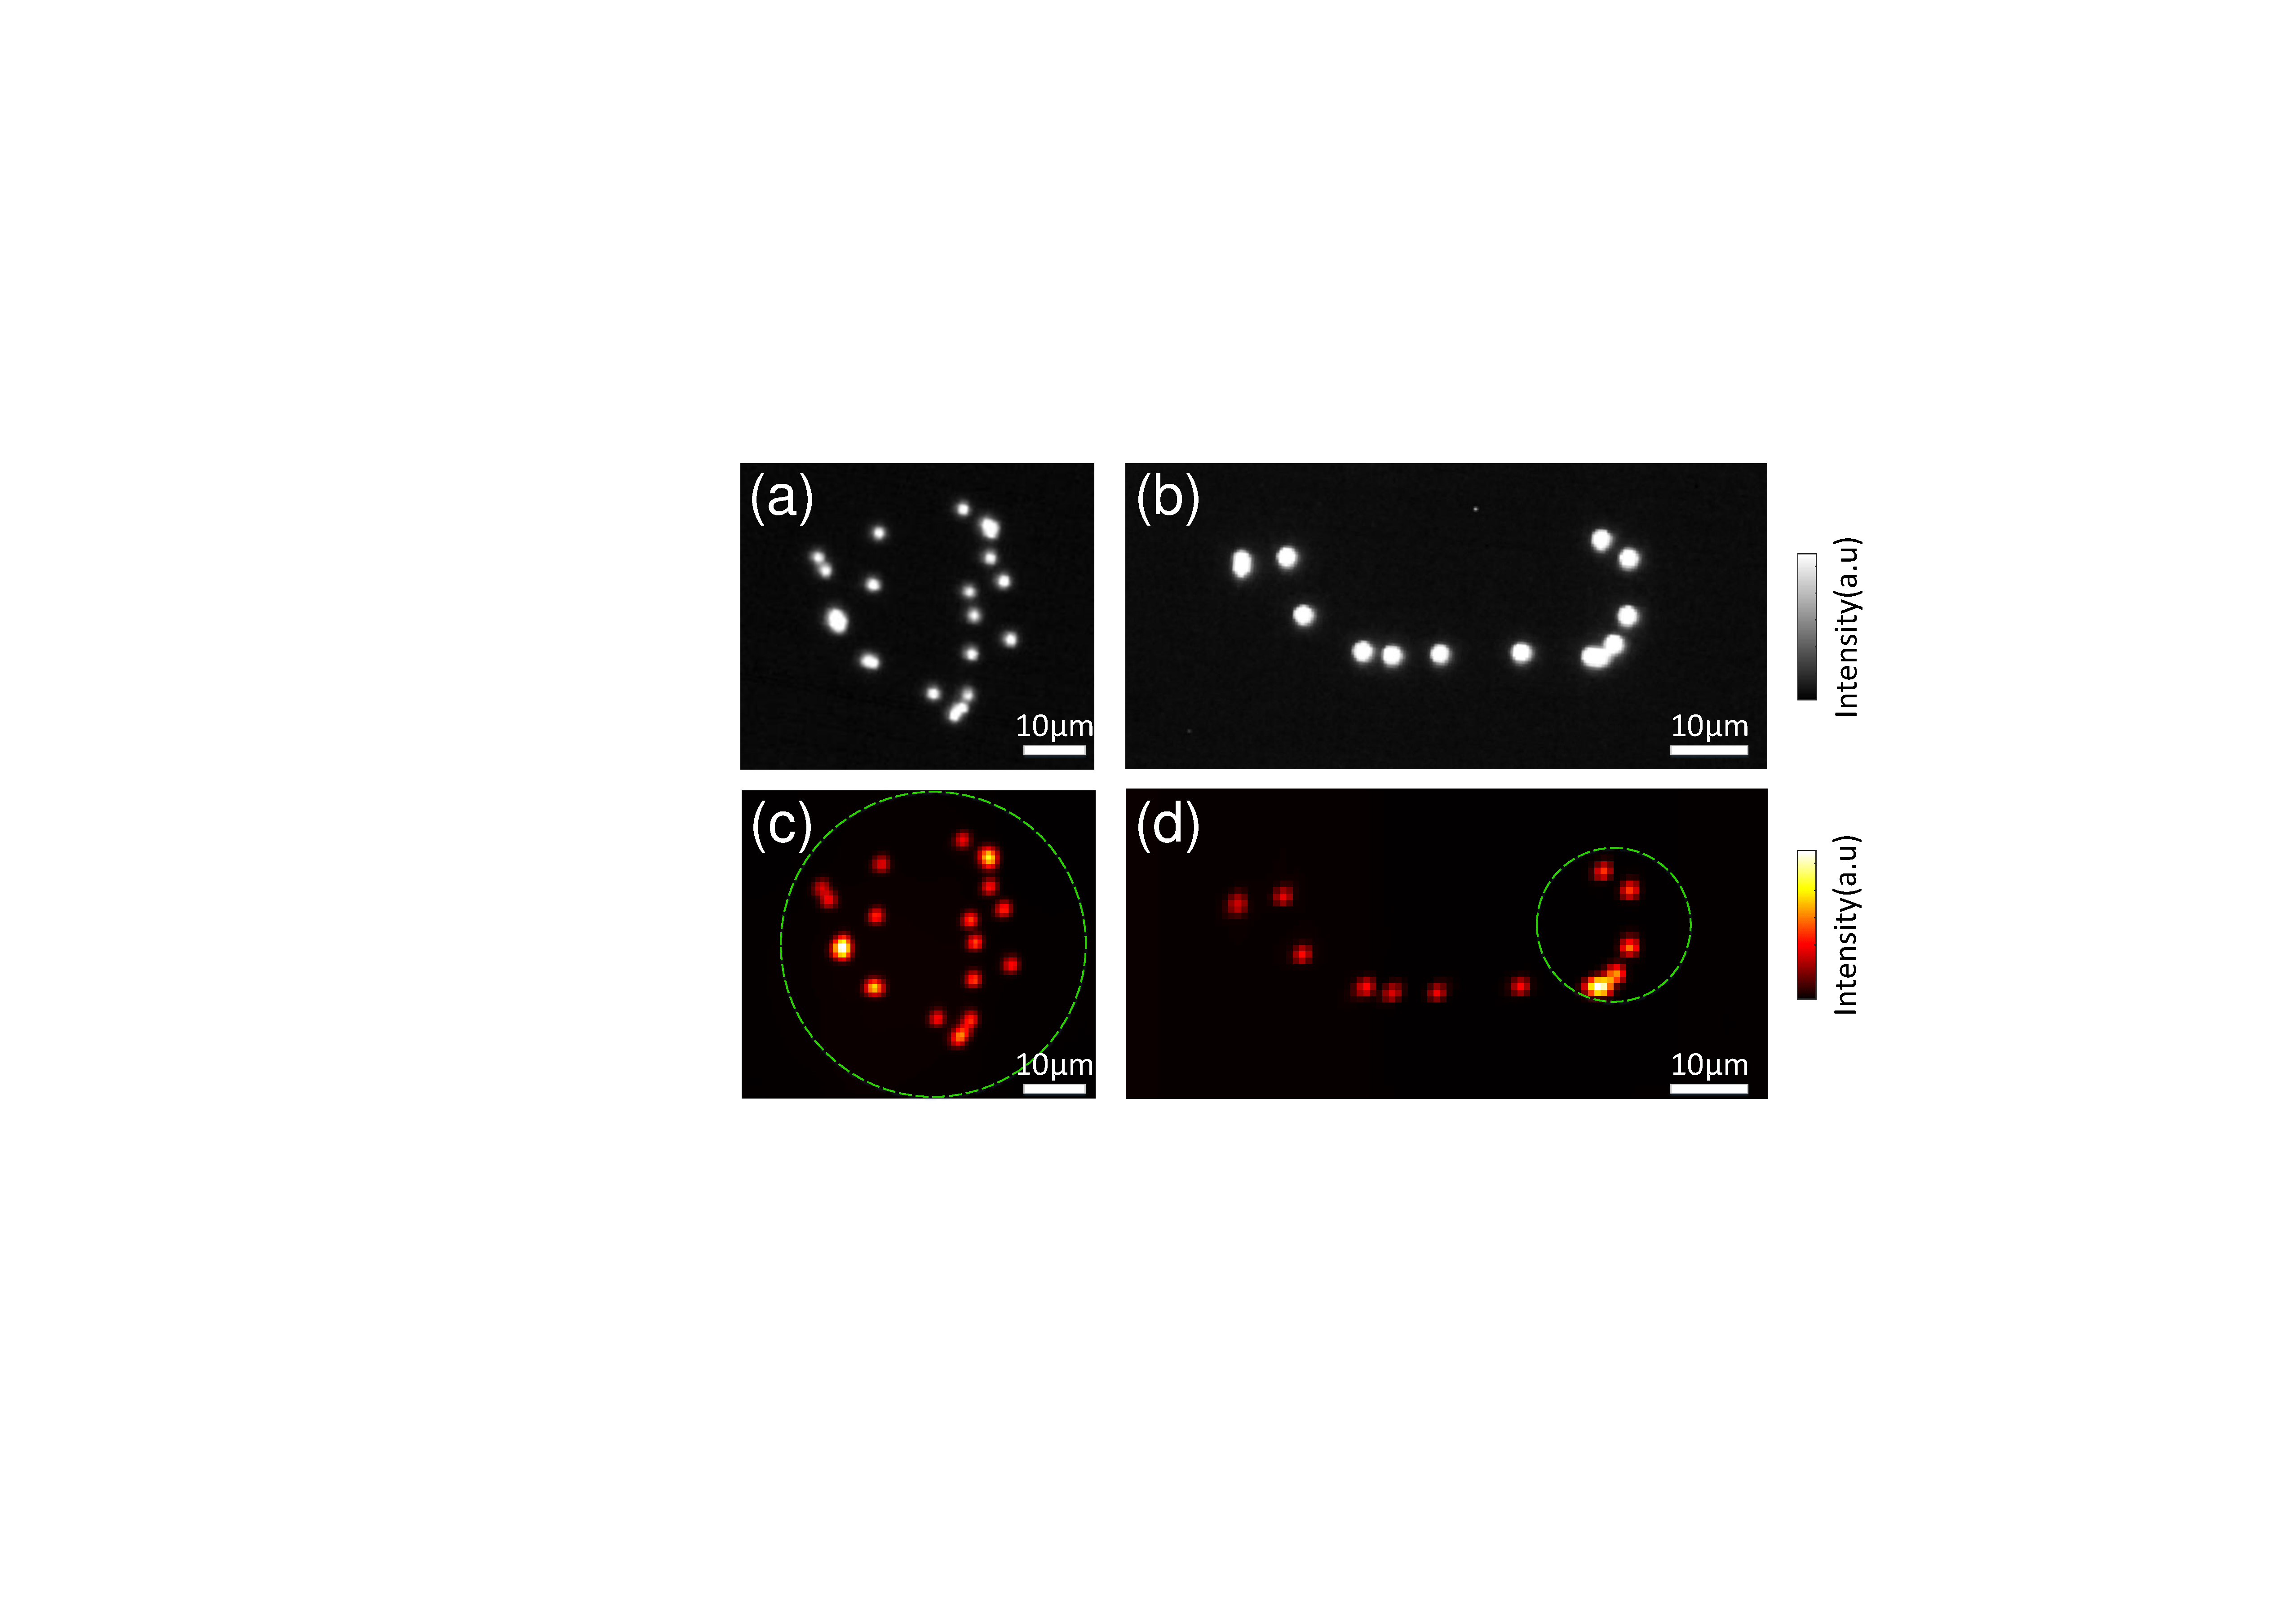
\includegraphics[scale=0.25]{C5.fig13}
	\caption{2D稀疏荧光目标透过散射介质成像实验结果}
	\label{fig:5.13}
\end{figure}

随后,我们又制作了不同的2D稀疏荧光目标,测试该成像方法的有效性和可重复性,实验结果如图\ref{fig:5.13}所示。图\ref{fig:5.13}(a)-(b)为没有散射介质的情况下记录的目标的荧光图像,(c)-(d)为使用NMF+FBR方法重建图像。(c)和(d)数据集所估计的NMF秩$\rho$为别为26和16。虚线圆圈表示OME范围。图\ref{fig:5.13}(d)所示的图像重建结果尺寸大约为OME范围的三倍。两组数据处理过程中,我们使用了的散斑数量$t$均为5120帧,相机的单次曝光时间分别为:$15ms$和$20 ms$。

从图\ref{fig:5.12}和\ref{fig:5.13}所展示实验结果可看出,我们的所提出的方法可以在没有约束的情况下重建跨越大约三倍OME范围的对象。

\subsection{复杂连续3D目标}

非稀疏、连续的物体在散射生物样本中很常见,这通常对通过散射介质方法进行的飞去亲成像提出了艰巨的挑战。 为了证明我们的技术也适用于非稀疏和连续目标,我们使用荧光染色的花粉种子形状目标,其重建图像如图\ref{fig:5.14}所示。图\ref{fig:5.14}(a)-(d)为无散射介质的情况下记录的不同花粉种子结构的荧光图像,(e)-(h)为使用 NMF+FBR方法重建图像。(e)-(h)数据集所估计的NMF秩$\rho$为别为68、85、45和55。虚线圆圈表示OME范围。两组数据处理过程中,我们使用了的散斑数量$t$均为5120帧,相机的单次曝光时间为$10 ms$。在非稀疏、连续的物体的重建过程中,所采用的重建过程严格按照图\ref{fig:5.12}所展示的流程。

\begin{figure}[htp]
	\centering
	\includegraphics[scale=0.13]{C5.fig14}
	\caption{非稀疏、连续复杂目标透过散射介质成像实验结果}
	\label{fig:5.14}
\end{figure}

从图\ref{fig:5.13}和图\ref{fig:5.14}可以看出,我们的方法不仅能够有效地重建稀疏点源目标,而且能够重建非稀疏、连续体目标。同时,仍有许多问题关于我们所提出地方法需要进行讨论,例如:散斑数量地选取、不同去卷积方法使用和NMF秩地选取等,将在下一部分进行详细讨论。

\section{实验分析与讨论}

\subsection{估计系统的秩}
在实验过程,我们需要对系统的秩$\rho$进行估计。如果我们未能准确的估计$\rho$将会对最终的重建结果造成何种影响?因此,我们研究了错误估计系统的秩$\rho$对我们重建质量的影响。我们实验性地选择了一个包含 10 个珠子的荧光物体。然后,我们采用不同的秩$\rho$对图像进行重建,秩$\rho$的范围从6到15。采用结构相似性指数度量 (Structural Similarity Index Metric,SSIM) \cite{Daoud2017} 用于量化重建的性能。如图\ref{fig:5.15} 所示,即使提出的$\rho$不完全准确,我们的技术也能够实现不同等级的重建。但是,低估$\rho$可能会导致在全局重建中丢失一些珠子。另一方面,高估$\rho$会产生混合模式,阻碍获得不同点光源之间相对位置信息。最后,必须考虑的是,随着点光源的数量越来越多,正确的估计变得越来越困难,但与此同时,这对最终重建的不利影响越来越小。还值得注意的是,稍微高估$\rho$通常时在实际实验和重建过程中被采用。低估系统的$\rho$会导致丢失目标点,稍微高估只会提供额外的指纹,这些额外的指纹不包含点源目标的位置信息,这些信息将在FBR过程中自动剔除。

\begin{figure}[htp]
	\centering
	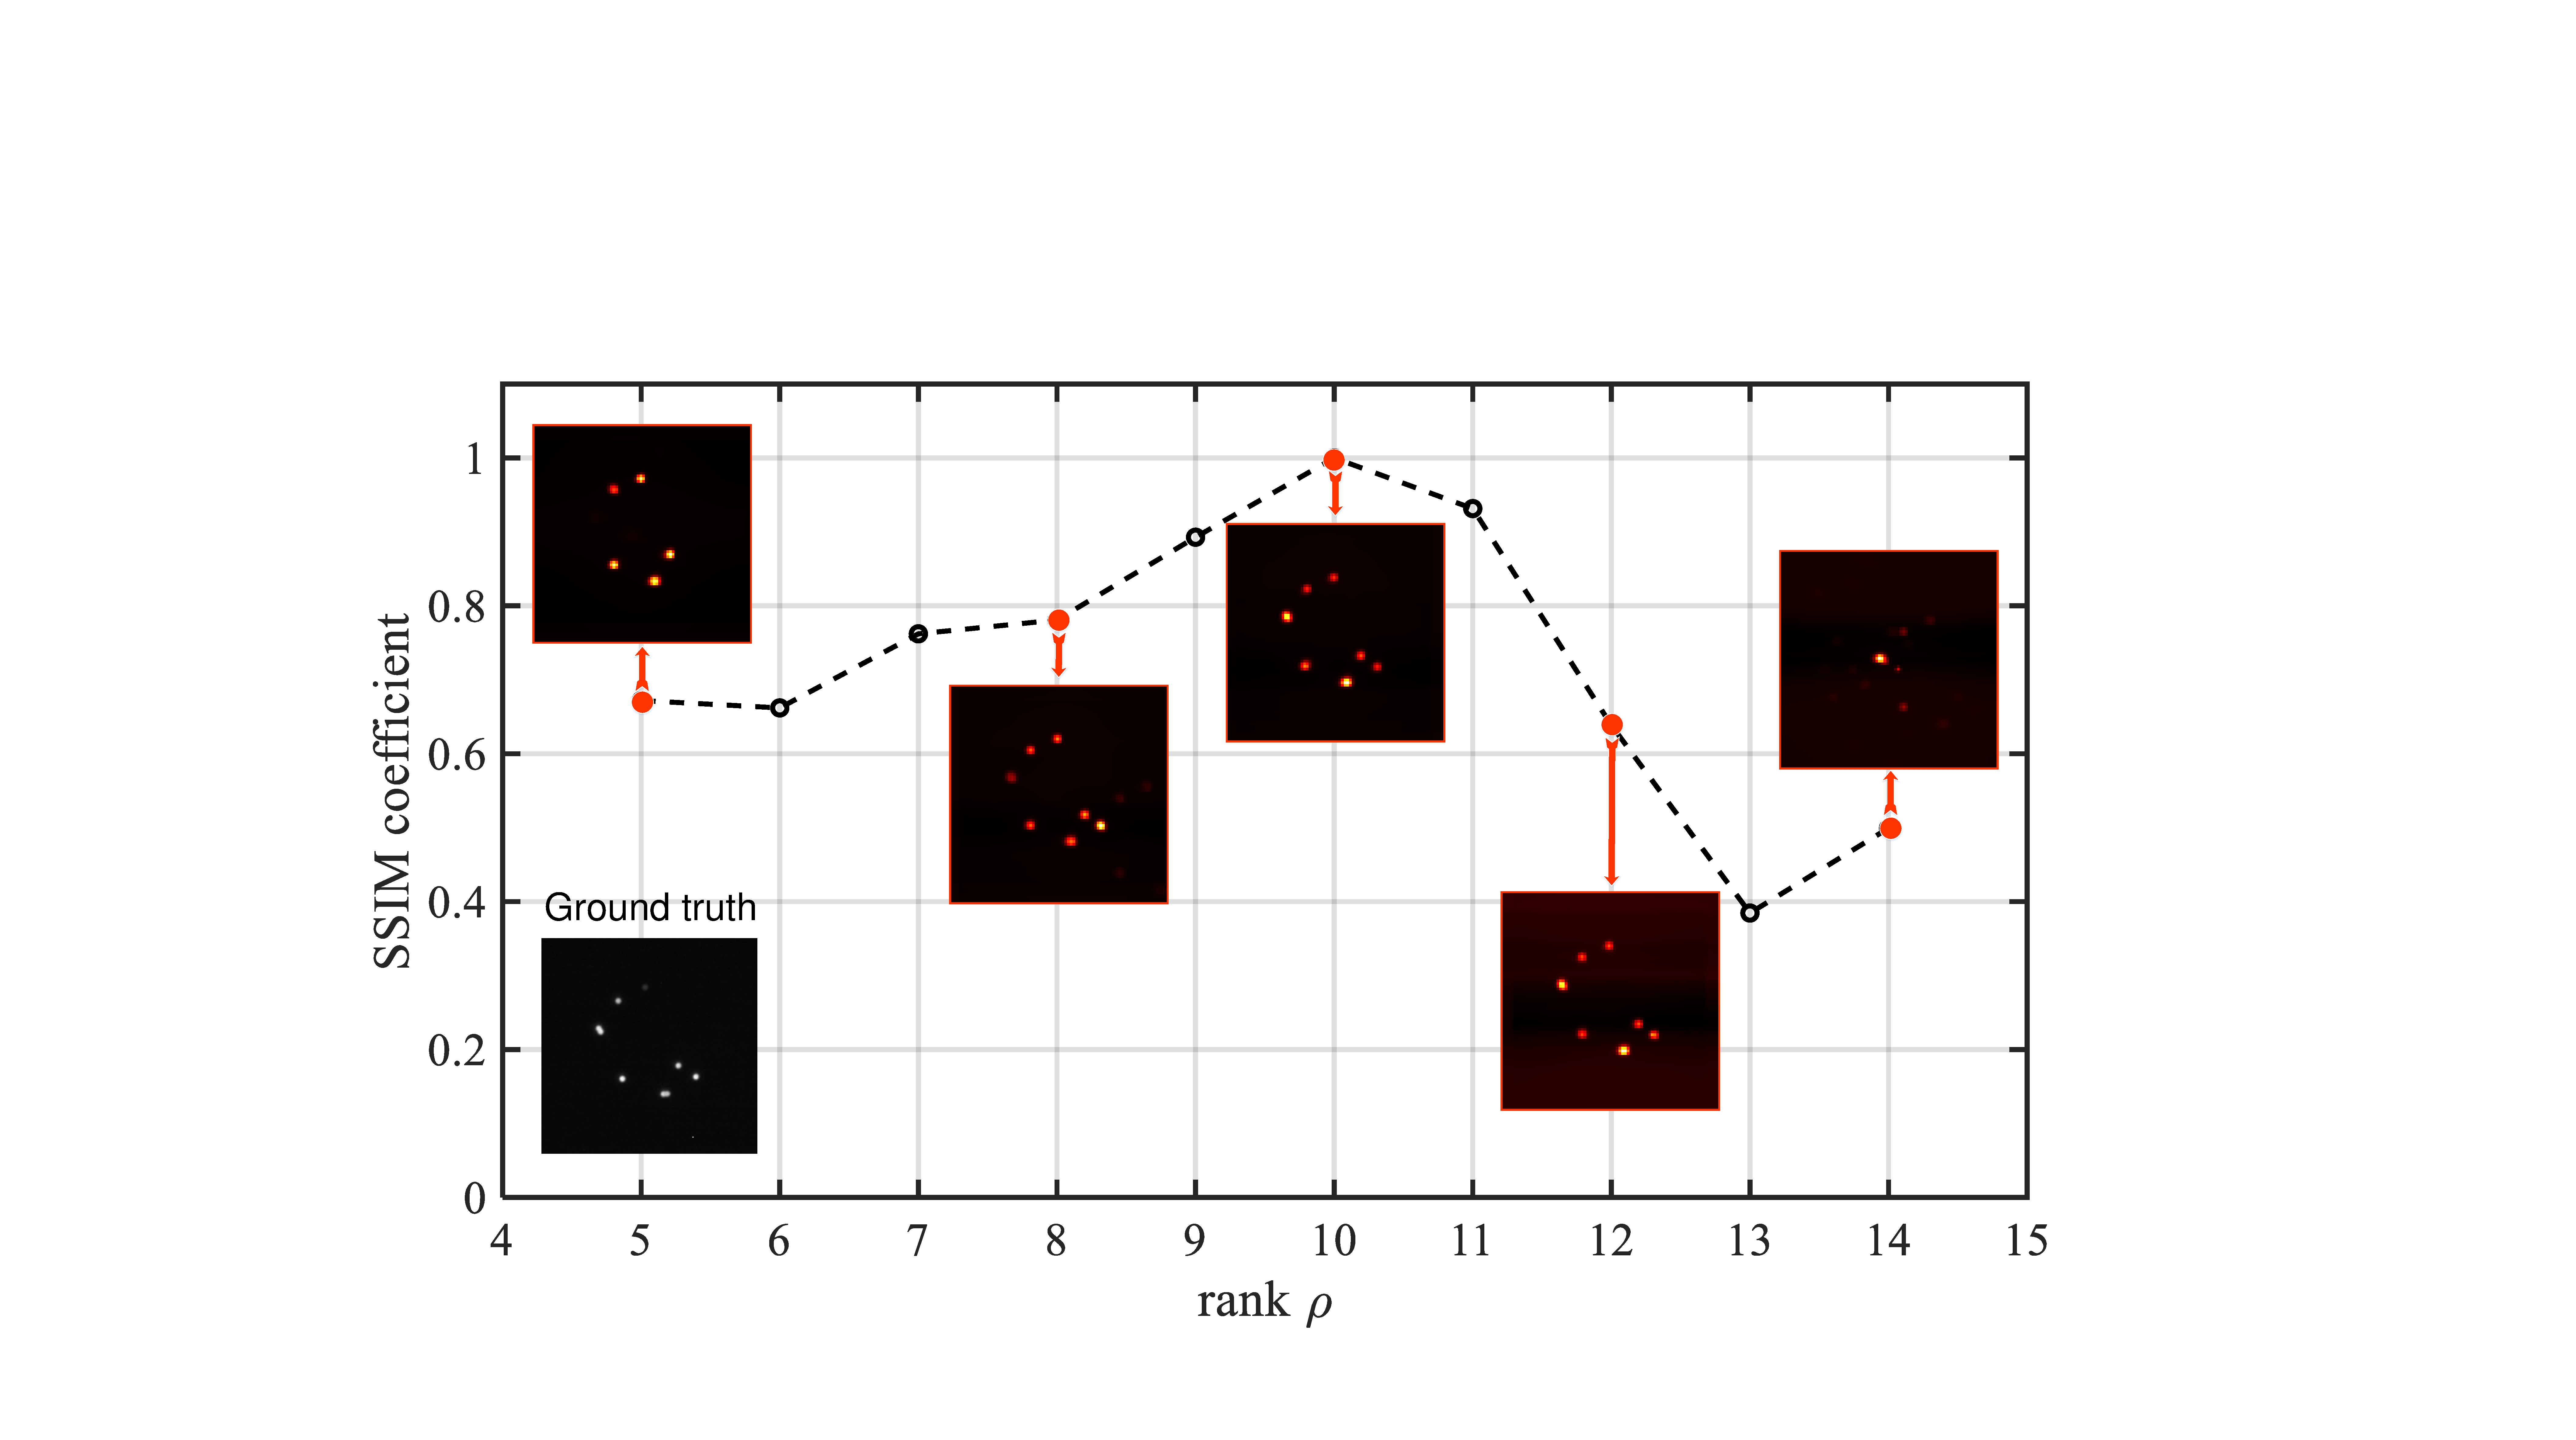
\includegraphics[scale=0.15]{C5.fig15}
	\caption{不同重建与参考图像之间的SSIM系数图}
	\label{fig:5.15}
\end{figure}

\subsection{OME范围}

为了证明我们的技术可以应用于OME范围以外的成像,测试了具有不同散射特性的介质。我们通过探索横向移动点光源(小荧光珠)时产生的散斑图案之间的相关性来估计每个散射介质的OME范围。随着源的移动,散斑图案之间的相关性逐渐降低,当距离大于OME范围时,相关性达到最小。测量这个距离可以估计每个扩散器的OME范围。图\ref{fig:5.16}为散射介质$\# 1$和散射介质$\# 2$荧光珠处于不同位置时散斑图案之间的相关系数,其中不同颜色表示来自不同的数据集,OME范围内的空间区域被标记为蓝色,OME范围外部被标记为红色。
如图所示\ref{fig:5.16},散射介质$\# 1$和散射介质$\# 2$分别对应的OME范围为$50 um$和$20 um$。当目标的尺寸小于OME范围时,该图像有可能通过散斑自相关的方式进行恢复(图\ref{fig:5.13}(a)对应的散斑介质$\# 1$);当图像的尺寸大于OME范围时,散斑自相关的方式无法恢复该图像(图\ref{fig:5.13}(b)对应的散斑介质$\# 2$,此目标的尺寸大约:$ 58 um \times 22 um $)。

\begin{figure}[htp]
	\centering
	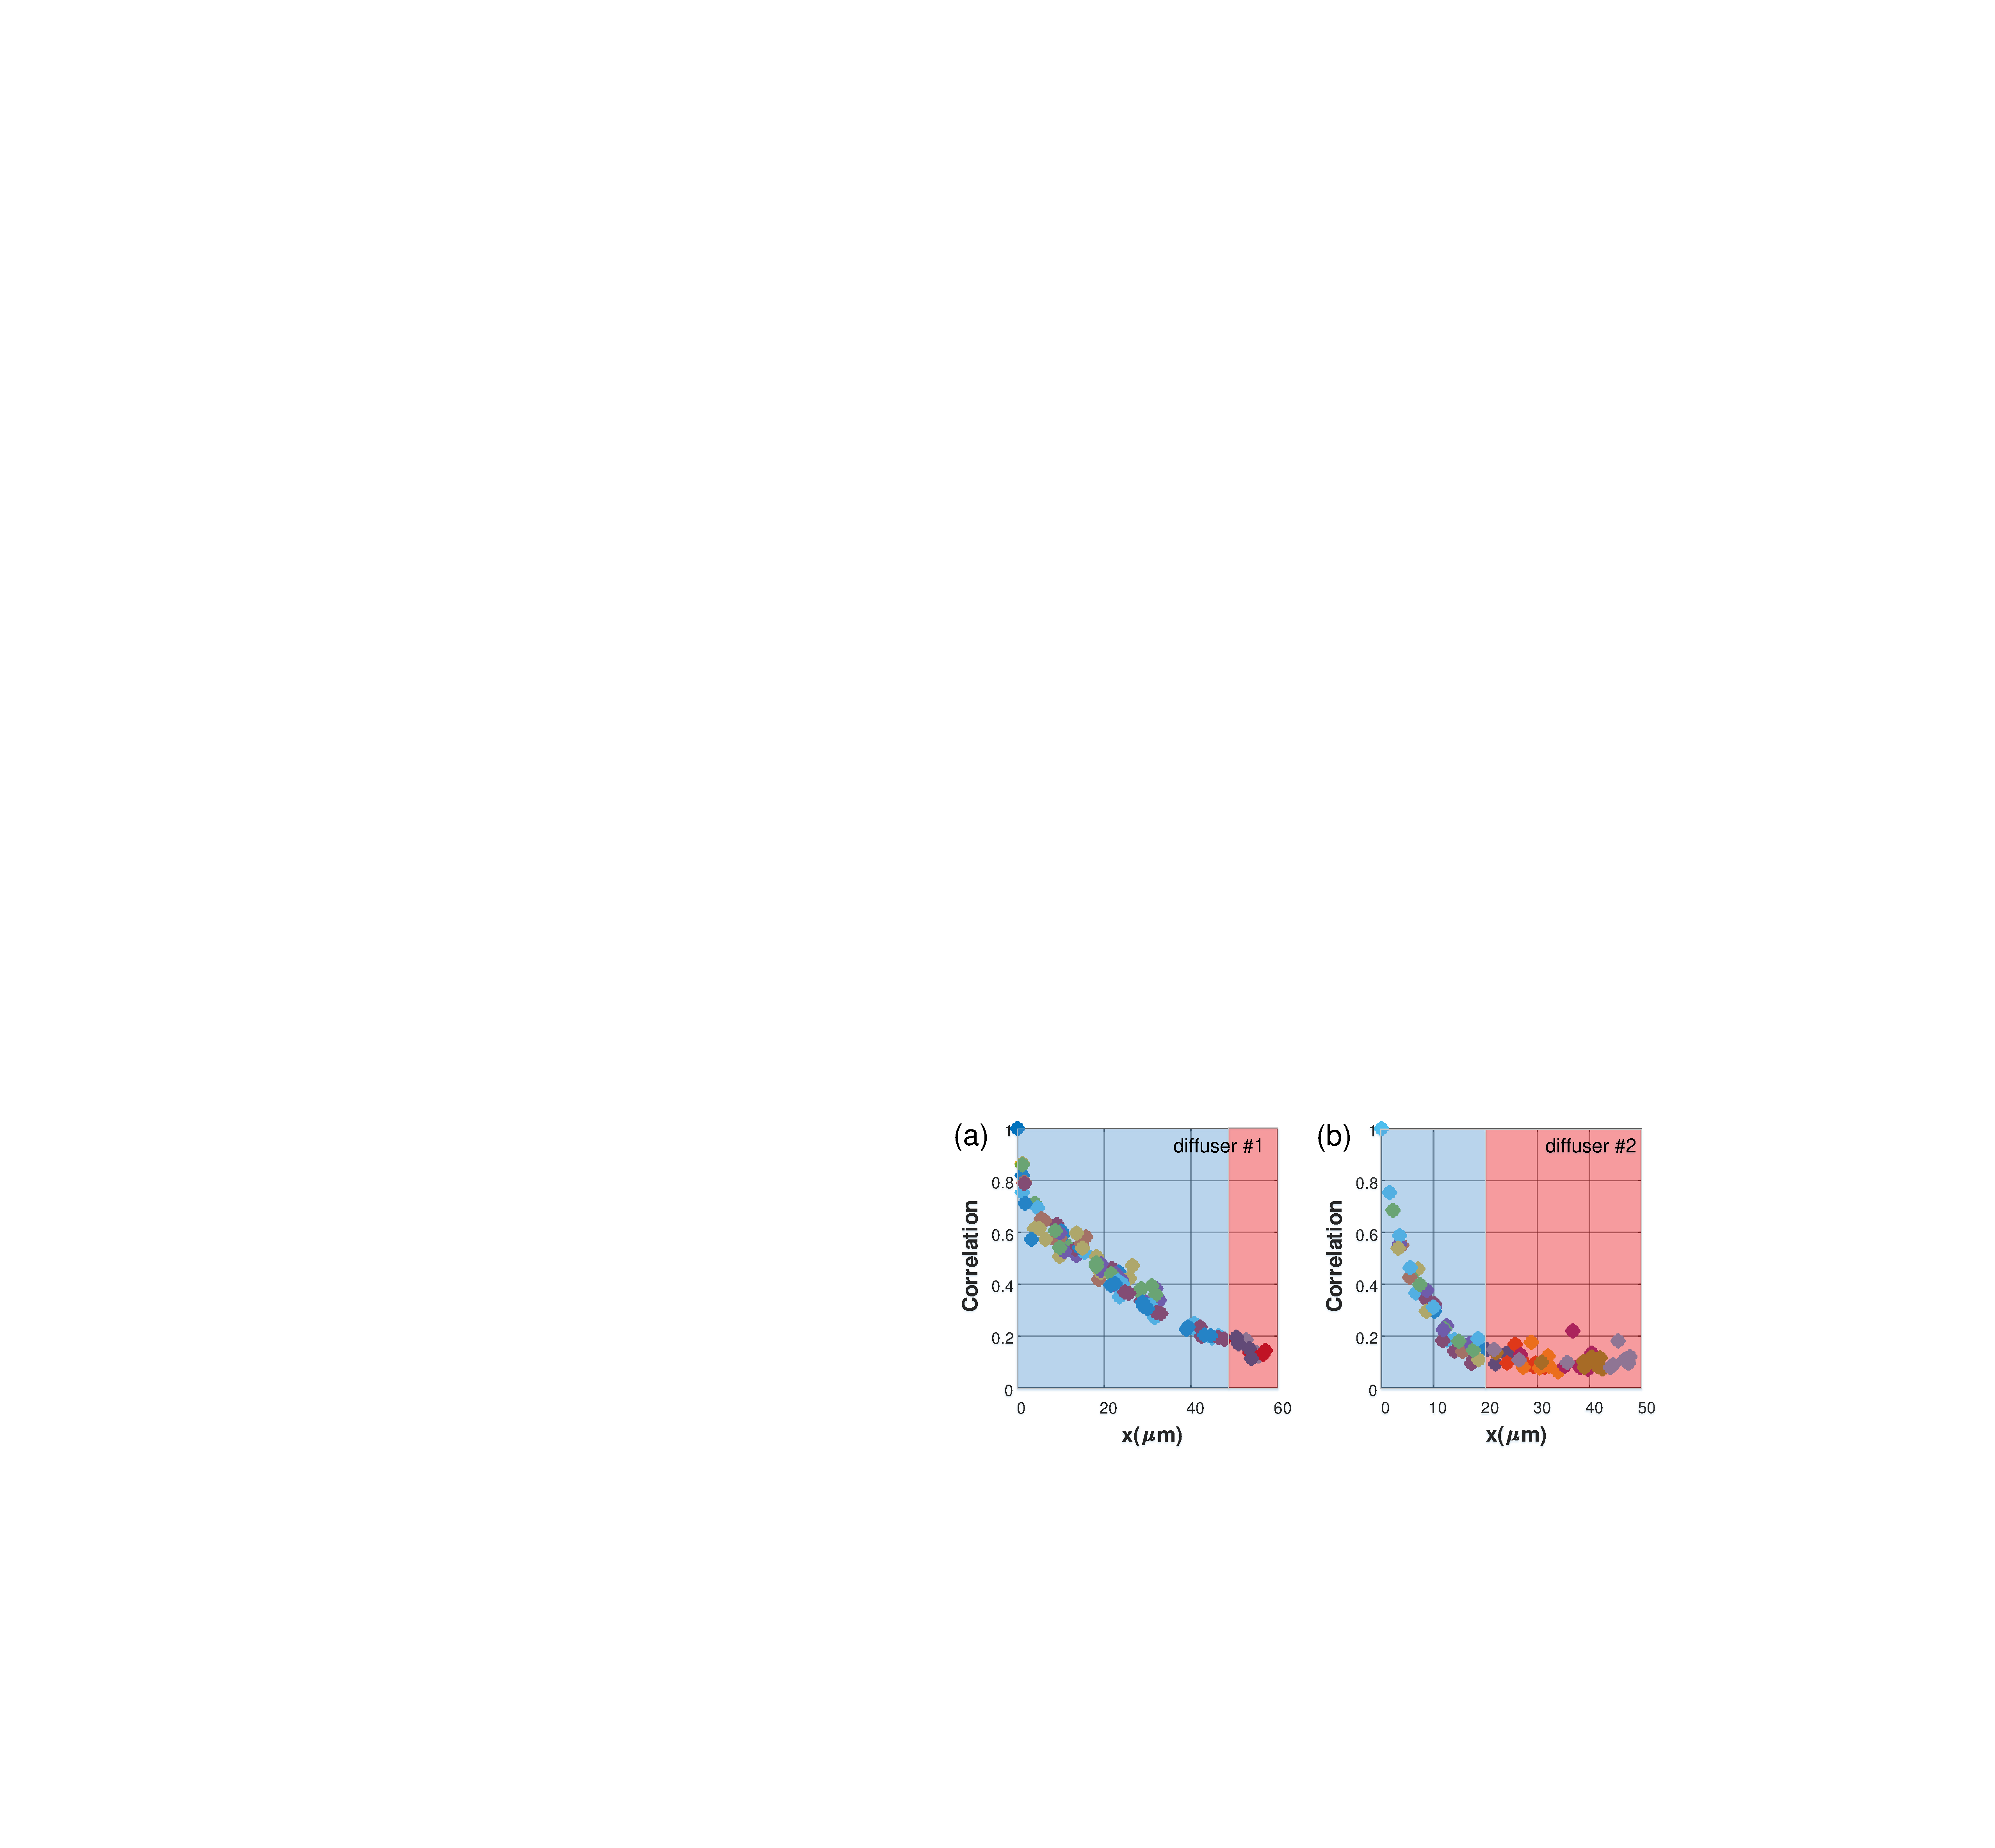
\includegraphics[scale=0.45]{C5.fig16}
	\caption{估计不同散射介质的OME范围}
	\label{fig:5.16}
\end{figure}

\subsection{FBR}

如上部分所述,只要不同的OME区域之间丁有一些重叠,FBR就可以重建整个对象。为了展示FBR的细节我们实验性地选择了一个包含3个荧光珠的荧光物体,并显示了成对反卷积 $o_{i,k}$ 和不同局部图像 $O_{k}$的各种结果。如图 \ref{fig:5.17}所示,点光源 $k$ 的 $O_{k}$ 可以通过选择 $w_{k}$ 作为PSF进行恢复。通过查看那些 $o_{i,k}$ 的最大值,可以检索指纹 $w_{i}$ 和 $w_{k}$ 之间的偏移 $\vec{r_{i,k}}$ ,如图\ref{fig:5.8}所示。实际上,来自OME范围之外的两个点光源的指纹不会提供它们点光源的相对位置信息(因为它们将完全不相关)。
因此,有必要推断指纹$w_{i}$和$w_{k}$是否在ME范围之内或之外。在我们的方法中,我们研究 $\alpha= \frac {max\{o_{i,k}\}} {max\{o_{k,k}\}}$ 作为相对距离的函数,其中 $max \{ o_{i,k} \}$ 代表 $o_{i,k}$ 的最大值。
一个给定的阈值 $\alpha_{tres}$ 被引入来评估它。例如,如果$\alpha$ 大于$\alpha_{tres}$,则$w_{i}$ 和$w_{k}$ 属于同一个OME范围。否则,它们属于不同的OME范围,无法检索它们的相对位置。图\ref{fig:5.18}为散射介质$\# 1$和散射介质$\# 2$荧光珠处于不同位置时散斑图案之间的$\alpha= \frac {max\{o_{i,k}\}} {max\{o_{k,k}\}}$曲线,其中不同颜色表示来自不同的数据集,OME范围内的空间区域被标记为蓝色,OME范围外部被标记为红色。

\begin{figure}[htp]
	\centering
	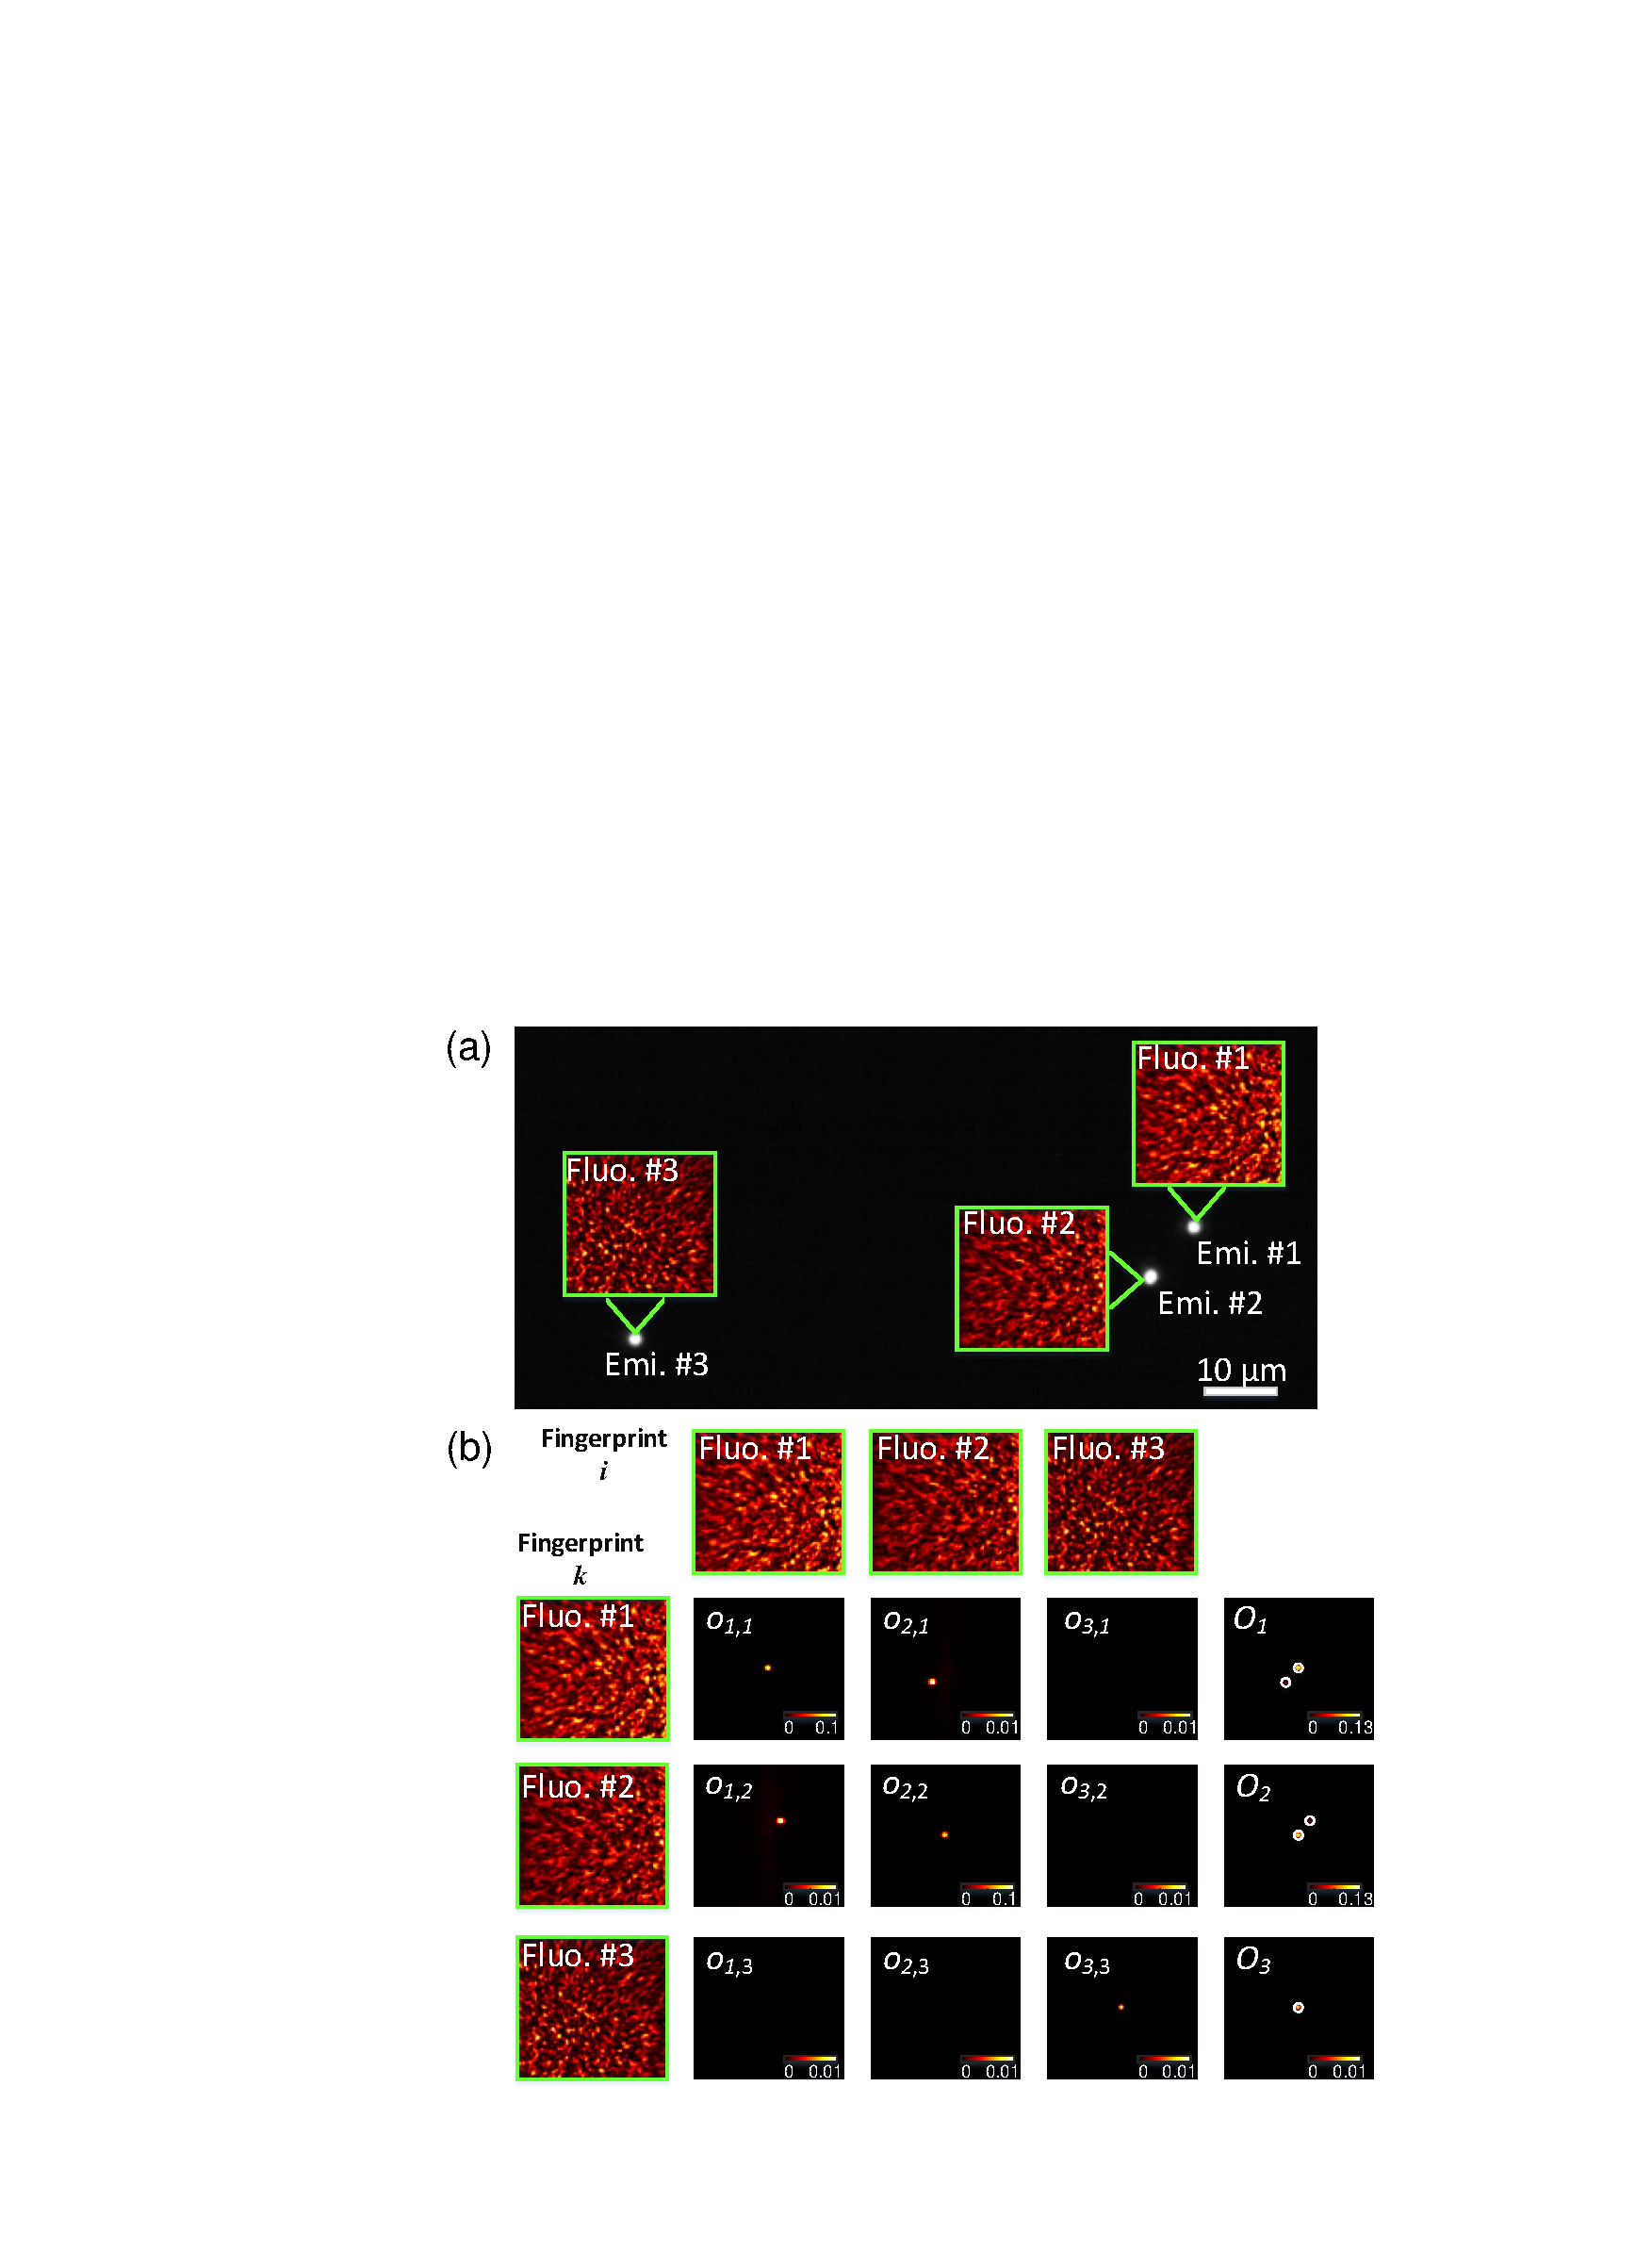
\includegraphics[scale=0.65]{C5.fig17}
	\caption{FBR细节信息}
	\label{fig:5.17}
\end{figure}

如图\ref{fig:5.18}所示,我们通过实验研究了成对反卷积的各种结果的最大值作为点光源之间距离的函数。本章所有展示的重建结果中, $\alpha_{tres}$ 设置为 $0.01$。

\begin{figure}[htp]
	\centering
	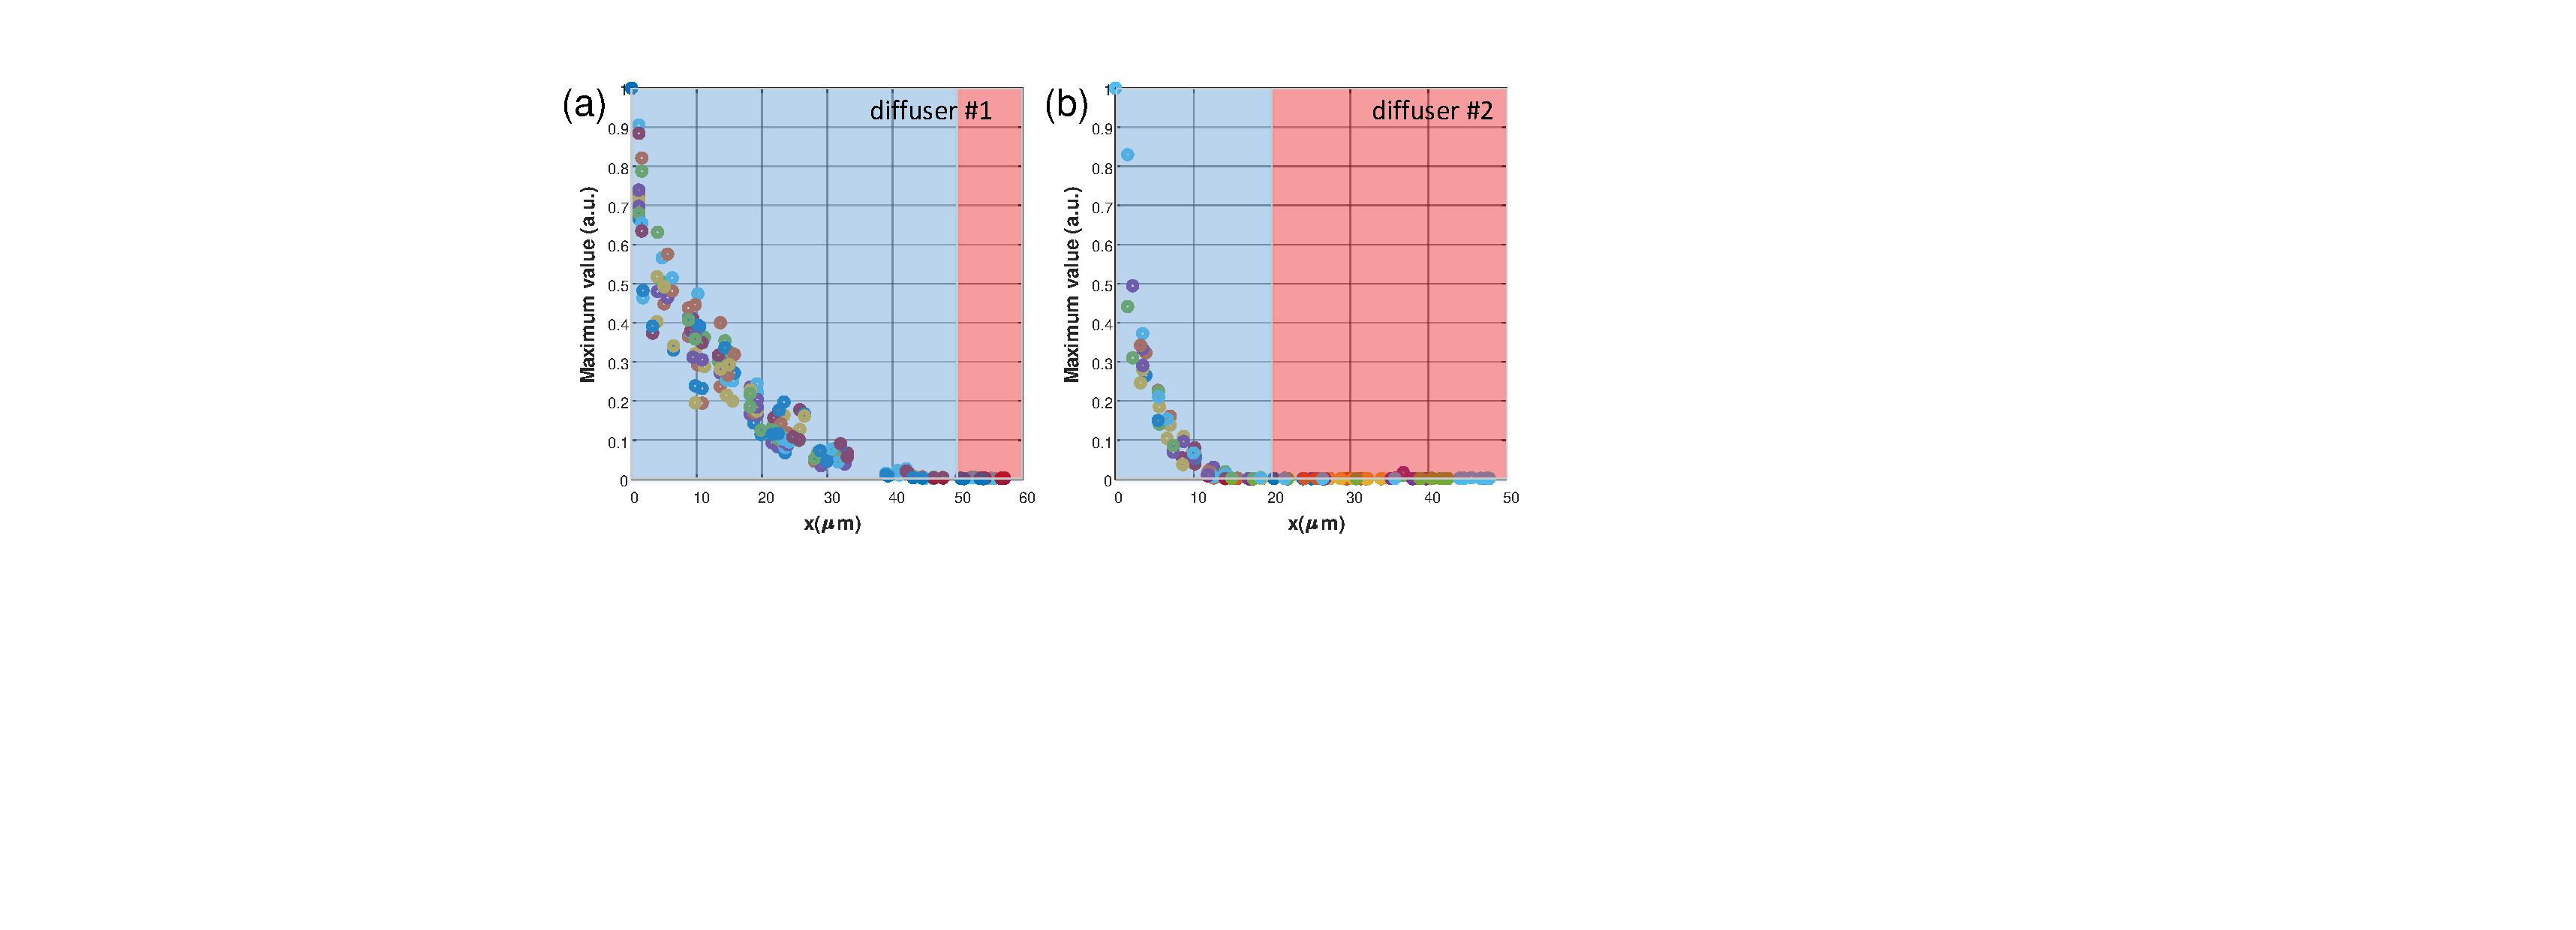
\includegraphics[scale=0.50]{C5.fig18}
	\caption{$\alpha= \frac {max\{o_{i,k}\}} {max\{o_{k,k}\}}$曲线图}
	\label{fig:5.18}
\end{figure}

\subsection{去卷积方和互相关方法的对比}

使用NMF算法重建散斑指纹后,可以通过查看其指纹之间的相关性来获得点光源之间的相对位置。对于OME范围内的点光源,其散斑指纹将是高度相关的横向偏移散斑图案,而超出OME范围的点光源将呈现不相关的指纹。传统上,横向偏移是通过在指纹之间进行互相关来测量的。当两者相关时,互相关处会出现一个峰值,其与中心的距离提供了它们之间的偏移。然而,这种方法存在一些缺点。主要问题来自指纹上的共同背景包络,即使在过滤后,也会在互相关中上升到背景,部分掩盖峰值(参见图\ref{fig:5.19}(d))。此外,当两个指纹不是$100 \%$相关时,峰值往往会变宽,从而影响定位精度。尽管可以对该结果进行后处理以“清理”互相关(参见图 \ref{fig:5.19}(e)),但针对不同的散射介质、OME范围和信号自动执行“清理”任务不是一个简单的过程。

选择去卷积而不是互相关的主要原因在于,我们无需额外的后处理步骤即可获得更清晰的结果,如图\ref{fig:5.19}所示。在图\ref{fig:5.19}中,(a)为无散射介质时所获取的图像,(b,c)物体中两个不同点光源的散斑指纹。(d)两个散斑指纹之间的原始互相关结果,(e)为原始互相关滤波后的结果,(f)为两个散斑指纹之间的去卷积结果,(g) 利用互相关的方法对图像进行重建(未滤波),(h)利用互相关的方法对图像进行重建(滤波后),(i)为利用本章所提出的重建方法的重建结果。我们选择的确切反卷积方法是基于我们系统的先验知识:对于通过横向偏移相关的两张图像,我们知道它们之间的反卷积结果应该是一个薄的$\delta$状尖峰,位于一定距离从横向移动距离给定的中心。我们所提出的重建方法能够有效的抑制噪声,而且有效的重建目标。为了定量的描述该算法对于噪声的抑制性能,假设我们拥有$p$个散斑指纹,需要进行$p^2$次成对全卷积运算或互相关运算,然后进行和。假设单次互相关运算所产生的噪声为$\varsigma$,进行加和运算后,最终的导致的噪声为$p^2 \cdot \varsigma$。相较于互相关运算,我们所提出的重建方法能够有效的对次项噪声进行抑制(参见图\ref{fig:5.19}(g-i))。

\begin{figure}[htp]
	\centering
	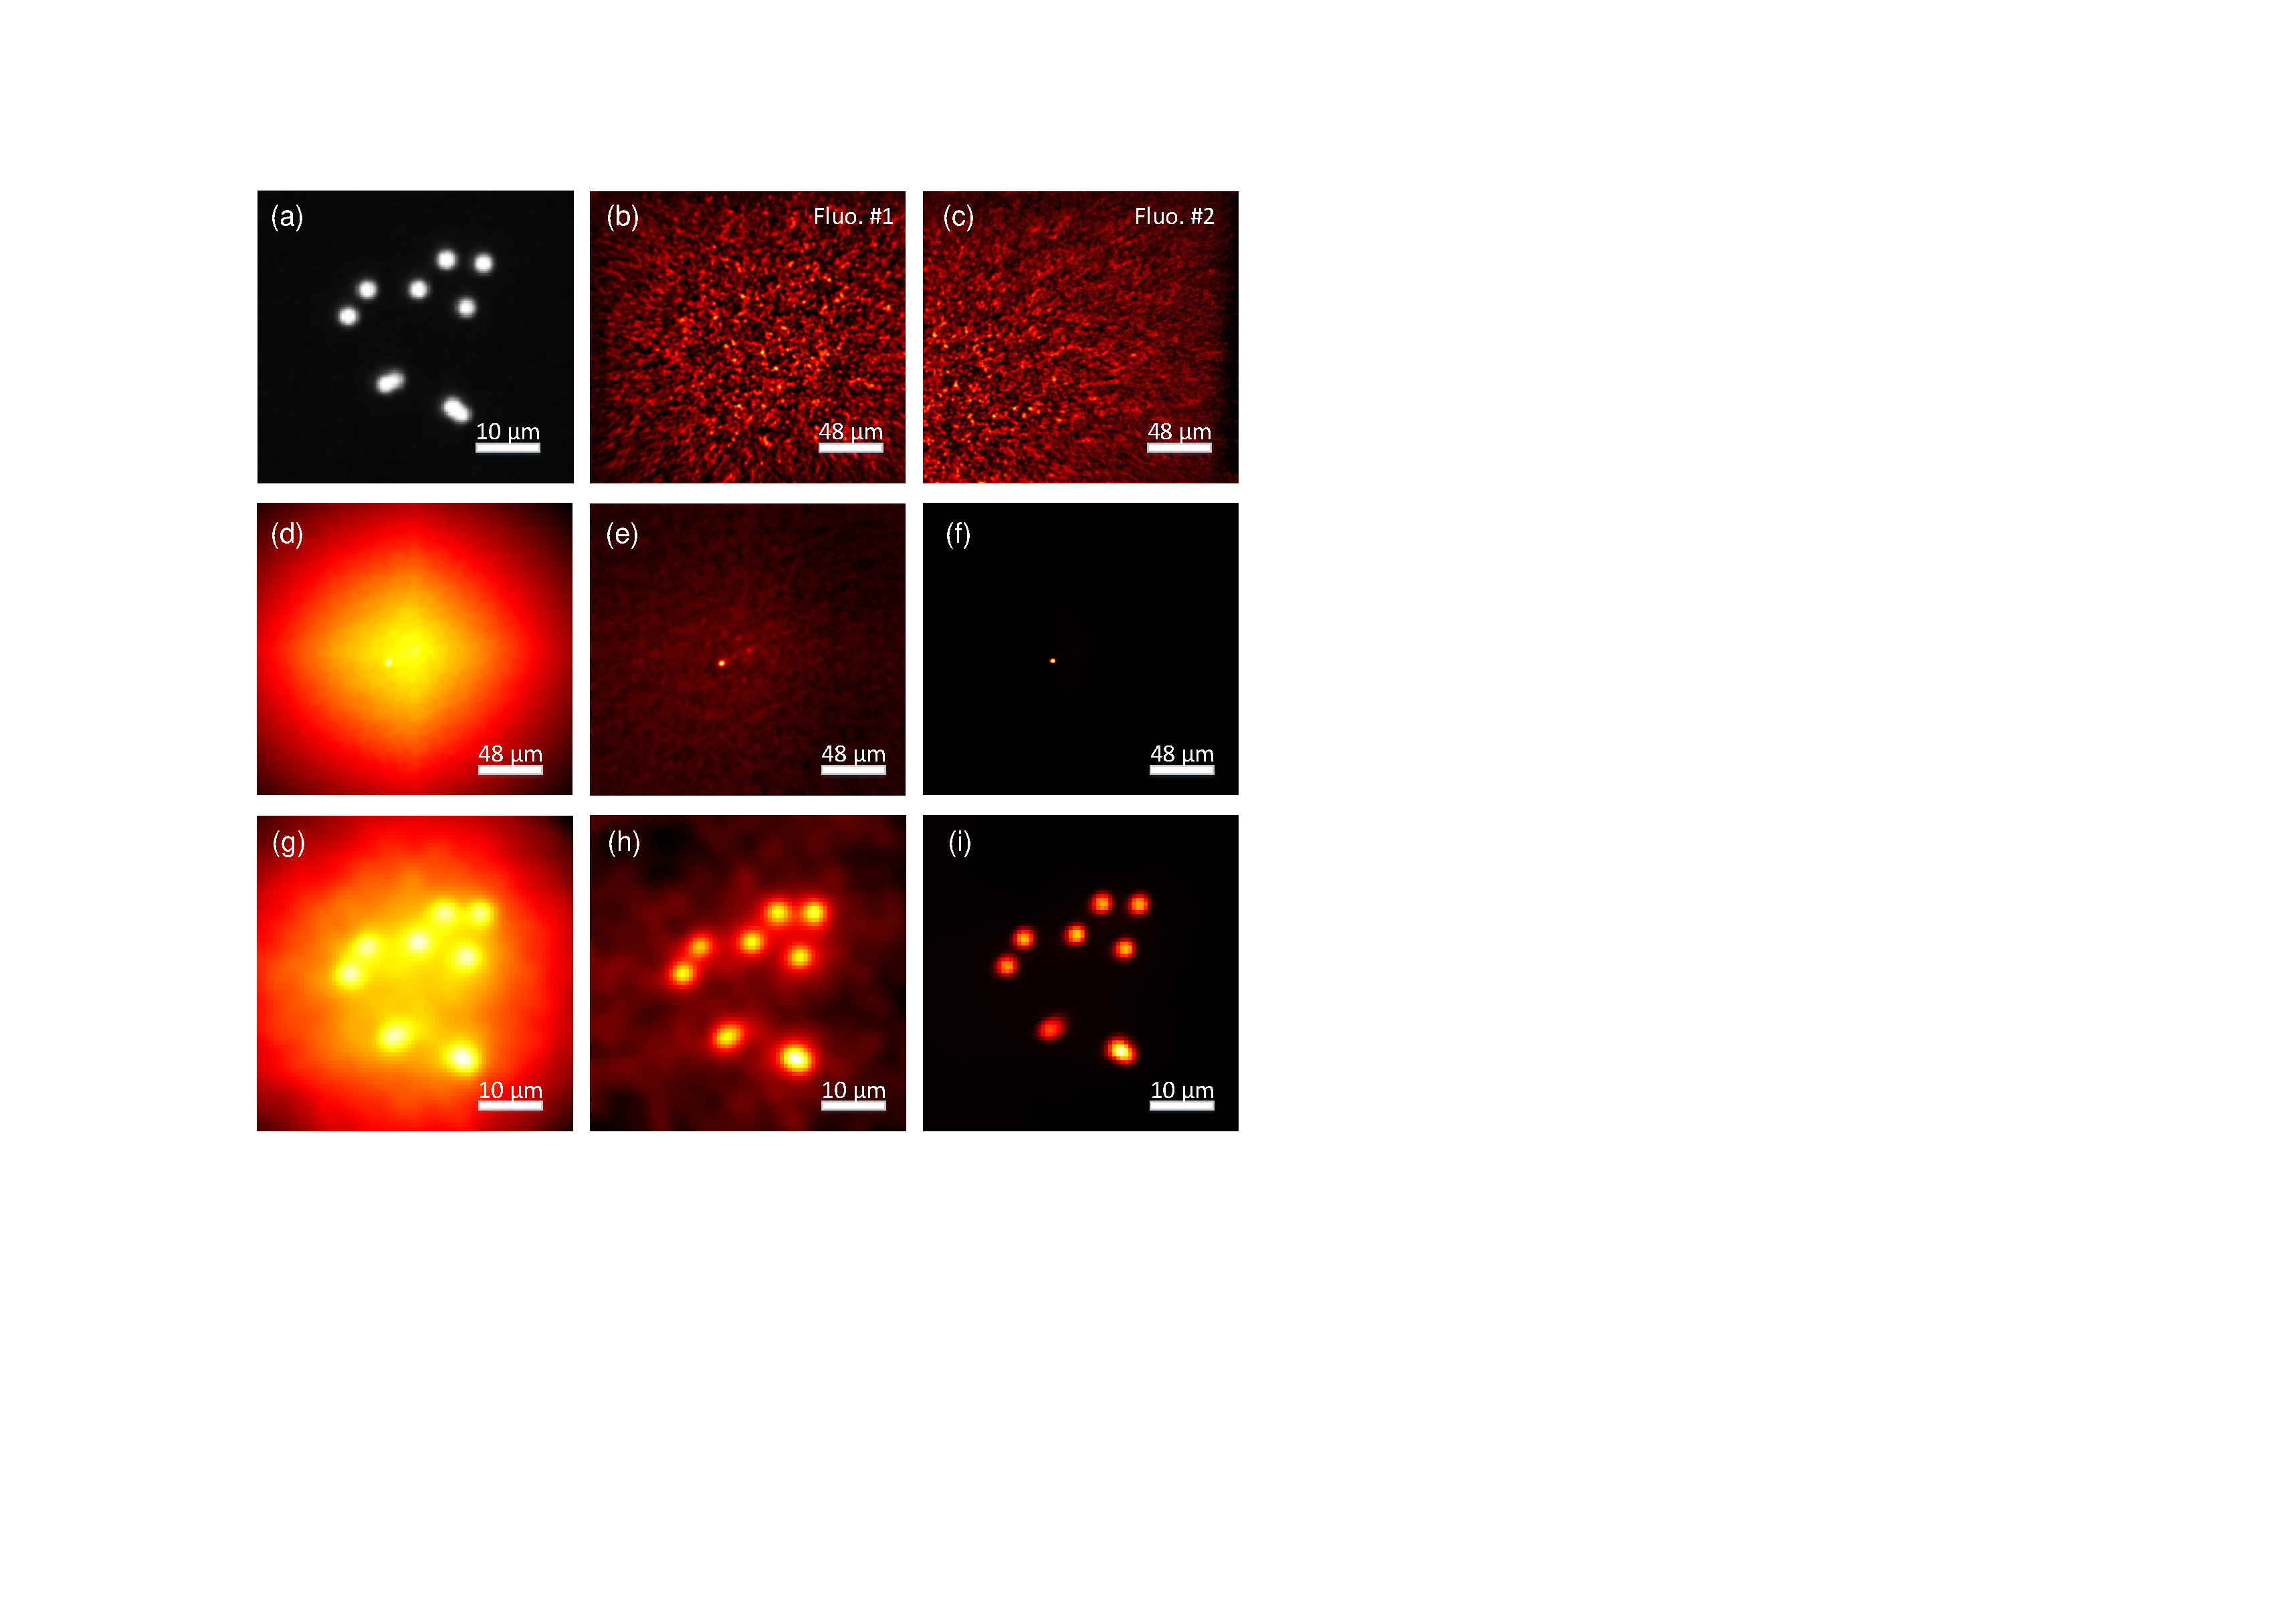
\includegraphics[scale=0.55]{C5.fig19}
	\caption{去卷积方和互相关方法的对比结果}
	\label{fig:5.19}
\end{figure}

\begin{figure}[htp]
	\centering
	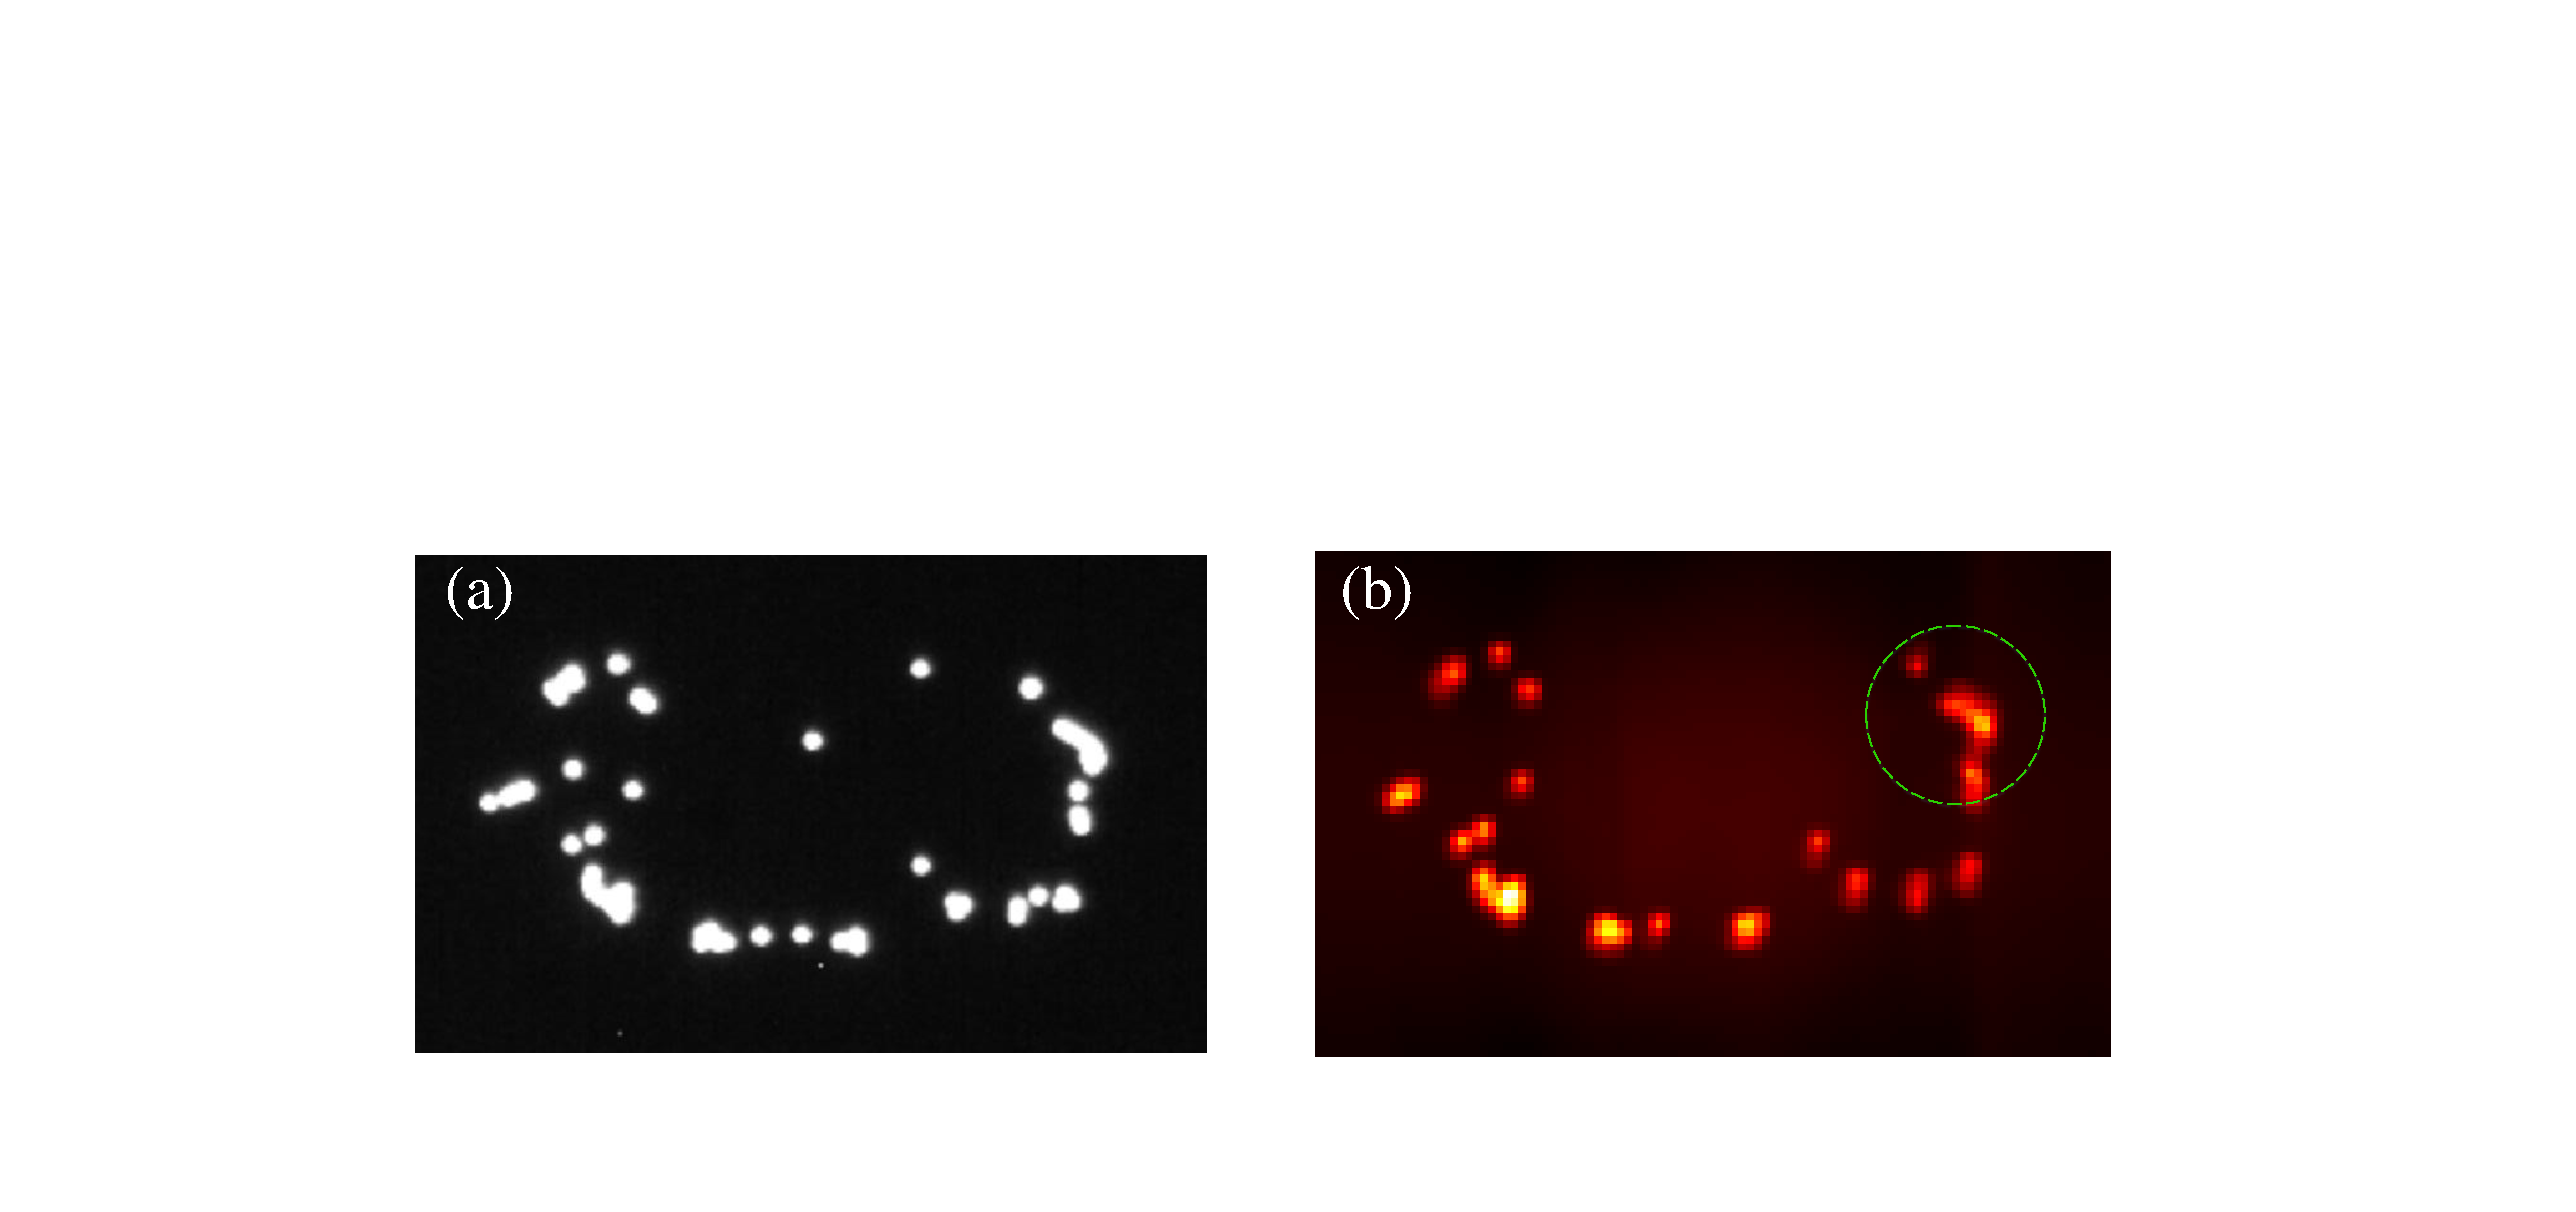
\includegraphics[scale=0.20]{C5.fig20}
	\caption{少量散斑照明时,稀疏目标的重建结果}
	\label{fig:5.20}
\end{figure}

\subsection{不同数量散斑对于重建结果的影响}

对于该重建方法,所需要的散斑数量也是值得考虑的问题之一。对于稀疏目标,利用数量较少的散斑,该方法可以有效的重建图像。对于复杂的连续目标,通常需要数量较多的散斑图像,才能有效的重建目标。本章所提出的非入侵图像重建中,首先需要利用NMF算法进行去混叠,实现散斑指纹的获取,数量越多的散斑输入有助于获取更加可靠的散斑指纹。为了证明,该方法在数量较少散斑情况下对于稀疏目标的重建有效性,进行了相应的实验。实验中,采用的散斑数量$t = 512$,其重建结果如图\ref{fig:5.20}所示。

对于所提出的重建方法而言,极具挑战的目标为复杂连续目标,于是我们进行实验,利用不同的散斑照明,实现连续目标的重建,重建结果如图\ref{fig:5.21}所示。图\ref{fig:5.21}中,(a)为无散射介质时,所获取的连续荧光目标的图像,(b)-(g)为使用不同数量的散斑照明时的重建结果。NMF所估计的秩$\rho$分别为:27,31,33,36,41和53对应(b)-(g)。理论上,随着输入散斑数量的增减,NMF的残差随着散斑数量的增加而减小,当残差越小时意味着NNF获取了更加可靠的散斑指纹。

\begin{figure}[htp]
	\centering
	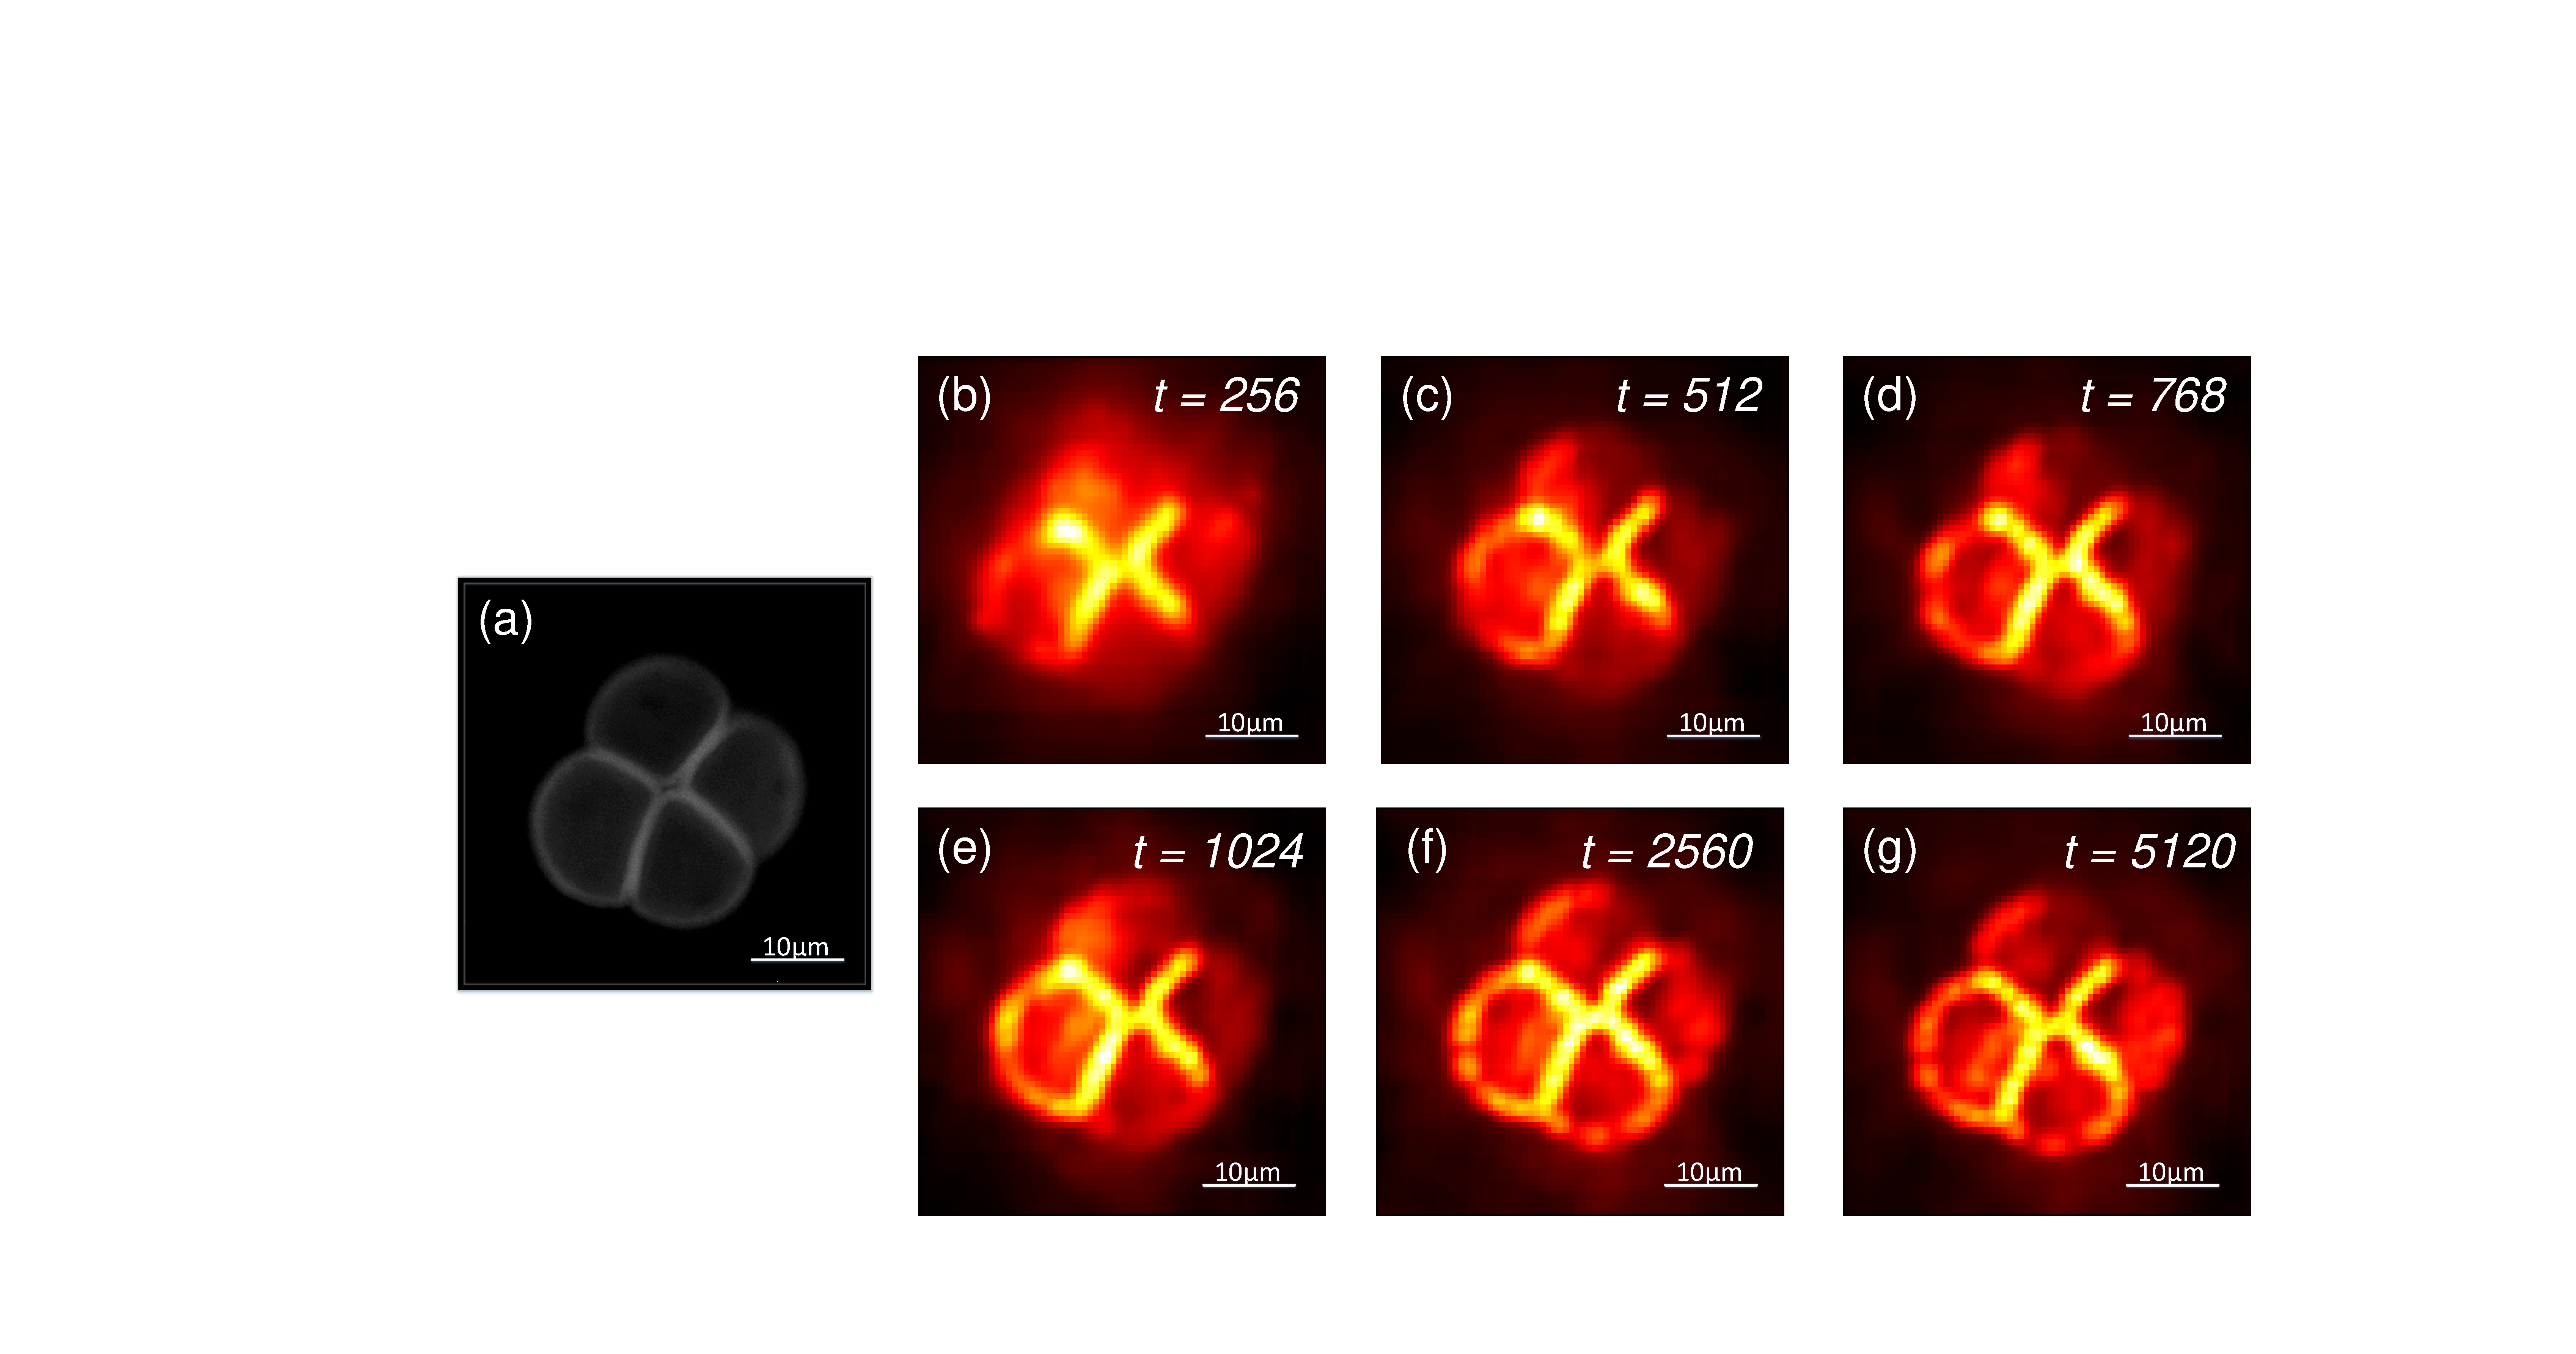
\includegraphics[scale=0.18]{C5.fig21}
	\caption{不同数量散斑照明时,连续目标的重建结果}
	\label{fig:5.21}
\end{figure}

\subsection{利用SLM产生随机照明}

如参考文献\cite{boniface_non_invasive_2020}所呈现方法,利用SLM提供随机照明,并记录不同随机照明时所SLM对应的相位分布,利用此信息可以实现非入侵的传输矩阵测量,进而实现聚焦和成像。本章所提出的非入侵透过散射介质成像方法也可以利用SLM提供照明,实现成像无需重新聚焦,实验结果如图\ref{fig:5.22}所示。图\ref{fig:5.22}中,(a)和(c)为分别无散射介质时,所获取的连续荧光目标的图像,(b)和(d)为分别对应于(a)和(c)的非入侵成像重建结果。NMF所估计的秩$\rho$分别为:14和53对应(b)和(d)。

\begin{figure}[htp]
	\centering
	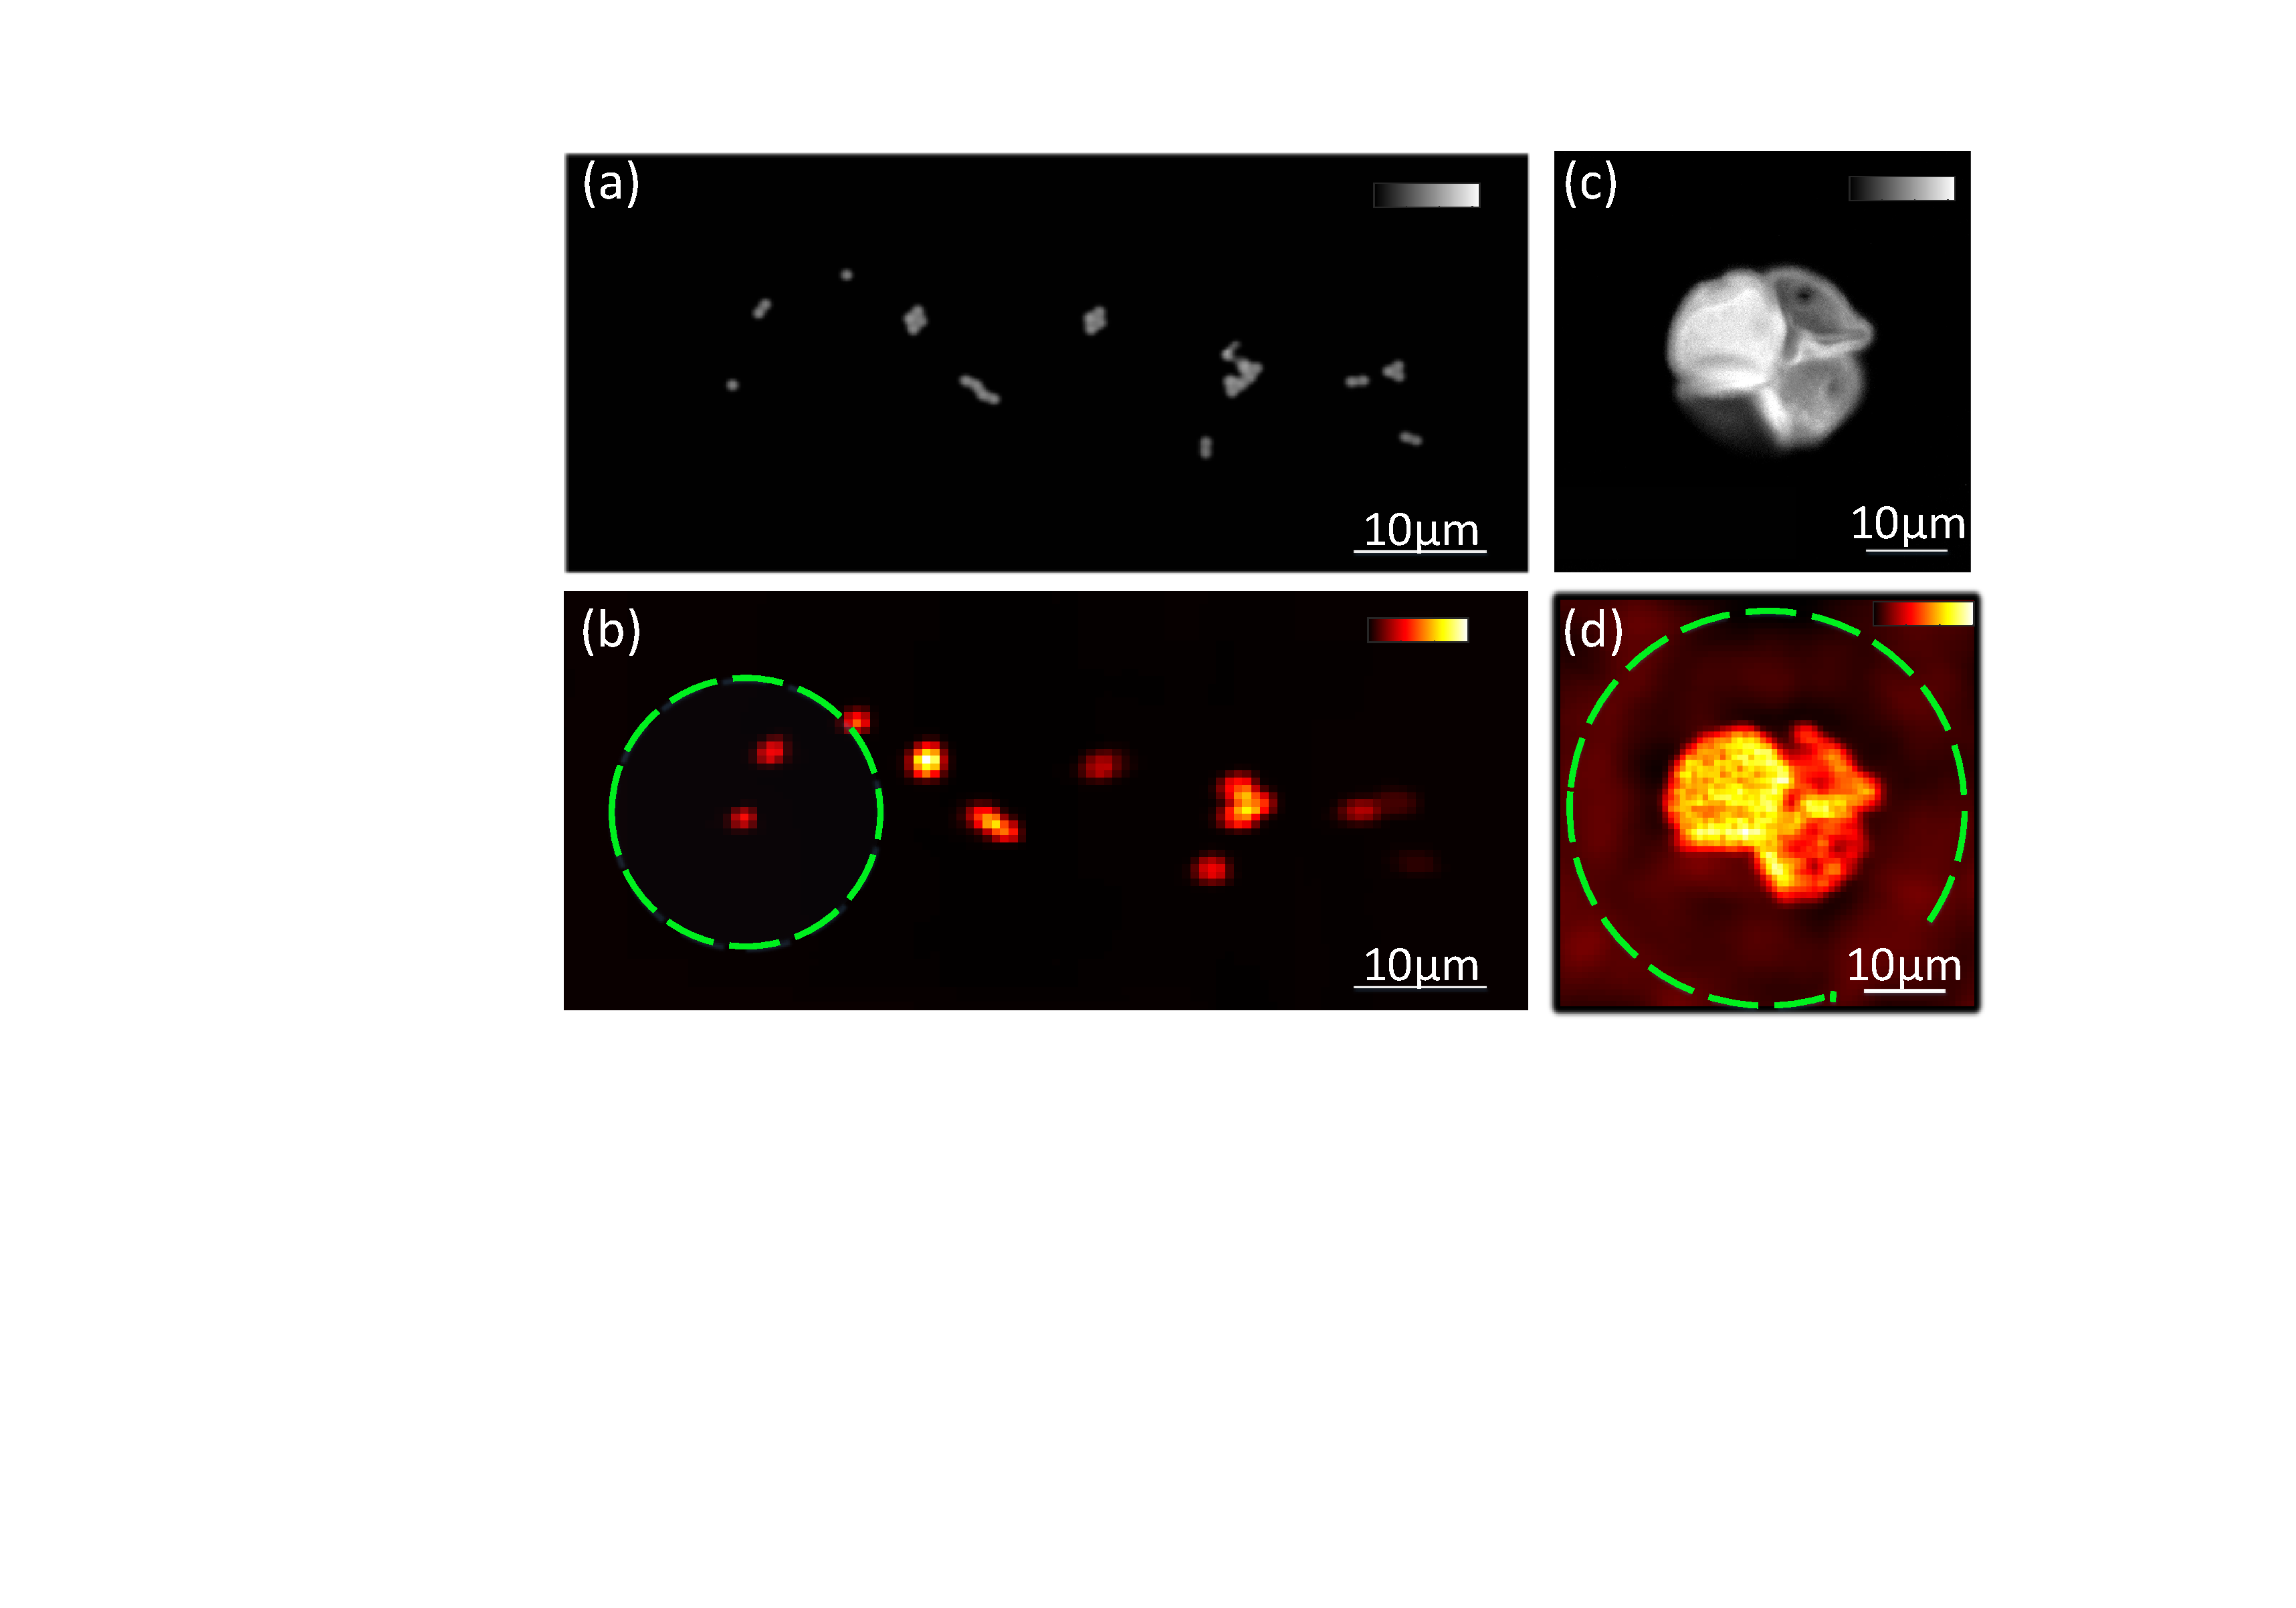
\includegraphics[scale=0.35]{C5.fig22}
	\caption{利用SLM提供随机照明时所重建的图像}
	\label{fig:5.22}
\end{figure}

\subsection{动态散射介质成像}

另一个重要的未来方向将是探索动态散射介质的方法来恢复其中的隐藏对象。在这方面,与基于光传输矩阵的技术相比,我们的技术不需要表征介质来检索图像,因为它仅依赖于随机照明产生的变化视频帧。然而,虽然我们的方法可以使用动态介质本身在嵌入对象上生成随机变化的照明模式,但NMF算法假设指纹在采集过程中不会改变。为了解决这个问题,应该探索考虑系统动力学的新的分解策略。如我们所了解到,NMF算法进行分解后,可以获得矩阵$W$和$H$。可以通过附加其他的约束条件,利用隐藏在矩阵$H$中的时间维度信息,进行更加复杂的图像重建或者动态散射介质成像条件下非入侵成像。

\section{本章小结}

在本章,我们展示通过利用指纹之间的相关性成功恢复隐藏对象。然而,我们相信,基于光谱OME或3D-OME,该技术可用于恢复多光谱或3D目标。另一个重要的未来方向将是探索动态散射介质的OME以通过它恢复隐藏对象。有趣的是,与基于光传输矩阵的技术相反,我们的技术不需要将光聚焦在物体上,并且仅依赖于随机照明产生的随机散斑图案,便可实现非入侵图像重建。另一个重要的一点是该技术的简单性,它不需要校准成像系统的PSF\cite{Antipa2018},并且可以在不需要昂贵的SLM的情况下实施。因此,我们的技术可以很容易地在各种散射介质和成像场景中实现。有必要强调的是,我们的方法与以前的自相关方法 \cite{bertolotti_non-invasive_2012,katz_non-invasive_2014} 相比,对于非稀疏连续目标的重建效果大大提升。

总之,本章展示了一种非侵入性技术,可以使用随机照明从低对比度荧光散斑中计算检索隐藏在散射介质后面的物体图像。我们已经证明我们的方法适用于稀疏目标(甚至超出OME范围)和复杂连续目标。重要的是,所提出的方法既不依赖弹道光也不使用波前整形,它适用于各种散射介质和物体。该技术的灵活性和稳健性,为强散射介质中进行深度荧光成像开辟了一条有希望的途径。最后,它可以推广到广泛的非相干对比度机制和照明方案。\textcolor{blue}{本章所解决的问题,超OME范围成像,但是不同OME范围之间互相存在重叠区域。在实际生物医学成像中,我们会遇到更复杂的情况,多目标位于多个OME范围,但是多个OME范围无重叠,此问题更具有挑战性,我们将在下一章节中进行展开讨论。}
